%fich.tex
%%%%%%%%%%%%%%%%%%%%%%%%%%%%%%%%%%%%%%%%%%%%%%%%%%%%%%%%%%%%%%%%%%%%%%%%
% Fco. Javier Bóhorquez Ogalla
% Descripción del documento:
	
%%%%%%%%%%%%%%%%%%%%%%%%%%%%%%%%%%%%%%%%%%%%%%%%%%%%%%%%%%%%%%%%%%%%%%%%


%%%%%%%%%%%%%%%%%%%%%%%%%%%%%%%%%%%%%%%%%%%%%%%%%%%%%%%%%%%%%%%%%%%%%%%%
%Clase de documento
\documentclass[12pt, spanish]{article}
%%%%%%%%%%%%%%%%%%%%%%%%%%%%%%%%%%%%%%%%%%%%%%%%%%%%%%%%%%%%%%%%%%%%%%%%


%%%%%%%%%%%%%%%%%%%%%%%%%%%%%%%%%%%%%%%%%%%%%%%%%%%%%%%%%%%%%%%%%%%%%%%%	
%Paquetes de lenguaje:
%%%%%%%%%%%%%%%%%%%%%%%%%%%%%%%%%%%%%%%%%%%%%%%%%%%%%%%%%%%%%%%%%%%%%%%%
\usepackage[utf8]{inputenc}
\usepackage[spanish]{babel}
%\usepackage[spanish, activeacute] {babel}	
%\usepackage[spanish]{babel} 				
%\usepackage[latin1]{inputenc}
%%%%%%%%%%%%%%%%%%%%%%%%%%%%%%%%%%%%%%%%%%%%%%%%%%%%%%%%%%%%%%%%%%%%%%%%


%%%%%%%%%%%%%%%%%%%%%%%%%%%%%%%%%%%%%%%%%%%%%%%%%%%%%%%%%%%%%%%%%%%%%%%%
%Paquetes para encabezados y pie de páginas
%%%%%%%%%%%%%%%%%%%%%%%%%%%%%%%%%%%%%%%%%%%%%%%%%%%%%%%%%%%%%%%%%%%%%%%%
\usepackage{fancyhdr}
%%%%%%%%%
% \pagestyle{fancy} %Si se cambia el estilo de página, antes de empezar 
	%el documento. Esto hace que el emcabezado y pie de página se 
	%quede separado del texto por una línea
%%%%%%%%%	
% \fancyhead{} % Límpia el texto que se está usando como encabezado
%%%%%%%%%
% \fancyhead[OPCIONES]{Encabezado}
	% OPCIONES:
		% L texto a la izquierda
		% C texto centrado
		% R texto a la derecha
		% E página par
		% O pagina impar
	%Ejemplo: 
		% fancyhead [LE] {"Doc. Latex"} 
			% Establece como emcabezado de las páginas pares "Doc Latex"
			% con alineacion a la izquierda
%%%%%%%%%			
% \fancyfoot[OPCIONES]{Píe de pag.}
	% OPCIONES:
		% L C R E O
	%Ejemplo
		% \fancyfoot[LE,RO]{\thepage} 
			% Establece como píe de pág. el número de página. con 
			% alineación a la izq en paginas pares y a la derecha en
			% las impares
%%%%%%%%%			
% \renewcommand{\headrulewidth}{0.4pt}
% \renewcommand{\footrulewidth}{0.4pt}
	% Fija el grosor de la la linea que separa el emcabezado y pie de pág
%%%%%%%%%
% Otros comandos:
%\lhead{}
%\chead{}
%\rhead{}
%\lfoot{}
%\cfoot{}
%%%%%%%%%%%%%%%%%%%%%%%%%%%%%%%%%%%%%%%%%%%%%%%%%%%%%%%%%%%%%%%%%%%%%%%%


%%%%%%%%%%%%%%%%%%%%%%%%%%%%%%%%%%%%%%%%%%%%%%%%%%%%%%%%%%%%%%%%%%%%%%%%
% Paquetes para tamaños y distancias
%%%%%%%%%%%%%%%%%%%%%%%%%%%%%%%%%%%%%%%%%%%%%%%%%%%%%%%%%%%%%%%%%%%%%%%%
\usepackage{anysize} 
%%%%%%%%%%%
% \marginsize{3cm}{2cm}{2cm}{2cm}
	% Controla los márgenes {izquierda}{derecha}{arriba}{abajo}. 
%%%%%%%%%%%%%%%%%%%%%%%%%%%%%%%%%%%%%%%%%%%%%%%%%%%%%%%%%%%%%%%%%%%%%%%%


%%%%%%%%%%%%%%%%%%%%%%%%%%%%%%%%%%%%%%%%%%%%%%%%%%%%%%%%%%%%%%%%%%%%%%%%
%Paquetes de carácteres especiales:
%%%%%%%%%%%%%%%%%%%%%%%%%%%%%%%%%%%%%%%%%%%%%%%%%%%%%%%%%%%%%%%%%%%%%%%%
\usepackage{dsfont}	
%Para representar conjuntos matematicos comunes: Z, N, R...
	% mathds{R}, mathds{N},...
%%%%%%%%%%%%%%%%%%%%%%%%%%%%%%%%%%%%%%%%%%%%%%%%%%%%%%%%%%%%%%%%%%%%%%%%

%%%%%%%%%%%%%%%%%%%%%%%%%%%%%%%%%%%%%%%%%%%%%%%%%%%%%%%%%%%%%%%%%%%%%%%%
%Paquetes para insertar gráficos
%%%%%%%%%%%%%%%%%%%%%%%%%%%%%%%%%%%%%%%%%%%%%%%%%%%%%%%%%%%%%%%%%%%%%%%%
\usepackage[dvips]{graphicx}
\DeclareGraphicsExtensions{.pdf,.png,.jpg} %solo para PDFLaTeX
%%%%%%%%%%%%%%%%%%%%%%%%%%%%%%%%%%%%%%%%%%%%%%%%%%%%%%%%%%%%%%%%%%%%%%%%

%%%%%%%%%%%%%%%%%%%%%%%%%%%%%%%%%%%%%%%%%%%%%%%%%%%%%%%%%%%%%%%%%%%%%%%%
%Paquetes de color:
%%%%%%%%%%%%%%%%%%%%%%%%%%%%%%%%%%%%%%%%%%%%%%%%%%%%%%%%%%%%%%%%%%%%%%%%
\usepackage{color}
%%%%%%%%%%%%%%%%%%%%%%%%%%%%%%%%%%%%%%%%%%%%%%%%%%%%%%%%%%%%%%%%%%%%%%%%
%Definición de colores:
\definecolor{gray97}{gray}{.97}
\definecolor{gray75}{gray}{.75}
\definecolor{gray45}{gray}{.45}
%%%%%%%%%%%%%%%%%%%%%%%%%%%%%%%%%%%%%%%%%%%%%%%%%%%%%%%%%%%%%%%%%%%%%%%%


%%%%%%%%%%%%%%%%%%%%%%%%%%%%%%%%%%%%%%%%%%%%%%%%%%%%%%%%%%%%%%%%%%%%%%%%
%Paquete de listado de código:
%%%%%%%%%%%%%%%%%%%%%%%%%%%%%%%%%%%%%%%%%%%%%%%%%%%%%%%%%%%%%%%%%%%%%%%%
\usepackage{listings}
%%%%%%%%%%%%%%%%%%%%%%%%%%%%%%%%%%%%%%%%%%%%%%%%%%%%%%%%%%%%%%%%%%%%%%%%
%Configuración del listado:
\lstset { 
	frame=Ltb,
     framerule=0pt,
     aboveskip=0.2cm,
     framextopmargin=0.3pt,
     framexbottommargin=0.2pt,
     framexleftmargin=0.3cm,
     framesep=0pt,
     rulesep=.1pt,
     tabsize=2,
     backgroundcolor=\color{gray97},
     rulesepcolor=\color{black},
     %
     stringstyle=\ttfamily,
     showstringspaces = false,
     basicstyle=\scriptsize\ttfamily,
     commentstyle=\color{gray45},
     keywordstyle=\bfseries,
   	%
     numbers=left,
     numbersep=1pt,
     numberstyle=\tiny,
     numberfirstline = false,
     breaklines=true,
}
%%%%%%%%%%%%%%%%%%%%%%%%%%%%%%%%%%%%%%%%%%%%%%%%%%%%%%%%%%%%%%%%%%%%%%%%


%%%%%%%%%%%%%%%%%%%%%%%%%%%%%%%%%%%%%%%%%%%%%%%%%%%%%%%%%%%%%%%%%%%%%%%%
%Indexado. Índice alfabeticos
\usepackage{makeidx}
\makeindex %para habilitar indices
%%%%%%%%%%%%%%%%%%%%%%%%%%%%%%%%%%%%%%%%%%%%%%%%%%%%%%%%%%%%%%%%%%%%%%%%
%Forma de uso:
% \index{clave} %Para crear un indice de materia
% Supongase que queremos meter en el indice alfabetico referencias a 
% las paginas donde se hace referencia a la clave Producto escalar
% en tal caso en cada una de las páginas pondremos \index{Producto escalar}
% \printindex %Para imprimir el índice alfabetico

% Es necesario una doble compilación del documento. La primera genera un 
% fichero.idx el cual tendremos que procesar con la aplicación makeindex
%tras procesarlo se creará un fichero.ind que contendra el código Latex 
% que se inserta en el documento original. 
% Tras la segunda compilación del documento original se sustituira el
% comando \printindex por el contenido del fichero.ind 

%Podemos cambiar el formato de la clave:
%Ejemplo     				&    	Entrada 		&	Comentario
%\index{hola}				&         hola, 1   	&	Entrada simple
%\index{hola!Pedro}			&		 Pedro, 3 	&	Subentrada bajo ‘hola’
%\index{Juan@\textsl{Juan}}  	&		Juan, 2    	&	Entrada con diseño                        
%\index{Pepa@\textbf{Pepa}}	&		Pepa, 7    	&	Igual que antes
%\index{Loli|textbf}		&		Loli, 3    	&	No de página con diseño                     
%\index{Soraya|textit}		&		Soraya, 5  	&	Igual que antes
%%%%%%%%%%%%%%%%%%%%%%%%%%%%%%%%%%%%%%%%%%%%%%%%%%%%%%%%%%%%%%%%%%%%%%%%


%%%%%%%%%%%%%%%%%%%%%%%%%%%%%%%%%%%%%%%%%%%%%%%%%%%%%%%%%%%%%%%%%%%%%%%%


%%%%%%%%%%%%%%%%%%%%%%%%%%%%%%%%%%%%%%%%%%%%%%%%%%%%%%%%%%%%%%%%%%%%%%%%
%Estilo de página
%%%%%%%%%%%%%%%%%%%%%%%%%%%%%%%%%%%%%%%%%%%%%%%%%%%%%%%%%%%%%%%%%%%%%%%%
%\textwidth 6.75in								  %ancho de texto
%\oddsidemargin -0.2in							%margen izquierdo 
\parskip 0.2in									%espacio parrafos
%%%%%%%%%%%%%%%%%%%%%%%%%%%%%%%%%%%%%%%%%%%%%%%%%%%%%%%%%%%%%%%%%%%%%%%%
\newenvironment{changemargin}[2]{%
\begin{list}{}{%
\setlength{\topsep}{300pt}%
\setlength{\leftmargin}{#1}%
\setlength{\rightmargin}{#2}%
\setlength{\listparindent}{\parindent}%
\setlength{\itemindent}{\parindent}%
\setlength{\parsep}{\parskip}%
}%
\item[]}{\end{list}}
%%%%%%%%%%%%%%%%%%%%%%%%%%%%%%%%%%%%%%%%%%%%%%%%%%%%%%%%%%%%%%%%%%%%%%%%
\usepackage{float}
\restylefloat{table}
\usepackage{placeins}
\usepackage{framed}
\usepackage{epsf}
%%%%%%%%%%%%%%%%%%%%%%%%%%%%%%%%%%%%%%%%%%%%%%%%%%%%%%%%%%%%%%%%%%%%%%%%

\usepackage{titlesec}

\setcounter{secnumdepth}{4}

\titleformat{\paragraph}
{\normalfont\normalsize\bfseries}{\theparagraph}{1em}{}
\titlespacing*{\paragraph}
{0pt}{3.25ex plus 1ex minus .2ex}{1.5ex plus .2ex}


%%%%%%%%%%%%%%%%%%%%%%%%%%%%%%%%%%%%%%%%%%%%%%%%%%%%%%%%%%%%%%%%%%%%%%%%	
%datos del documento
\author{Casos de uso \\\\\ Fco. Javier Bohórquez Ogalla}						%autor
\date{}														%fecha

\title{ 
\begin{center}

\includegraphics[scale=0.5]{logo-doc.png}
\end{center} 
}
%%%%%%%%%%%%%%%%%%%%%%%%%%%%%%%%%%%%%%%%%%%%%%%%%%%%%%%%%%%%%%%%%%%%%%%%

%%%%%%%%%%%%%%%%%%%%%%%%%%%%%%%%%%%%%%%%%%%%%%%%%%%%%%%%%%%%%%%%%%%%%%%%
%Documento:
%%%%%%%%%%%%%%%%%%%%%%%%%%%%%%%%%%%%%%%%%%%%%%%%%%%%%%%%%%%%%%%%%%%%%%%%
\begin{document}

\maketitle
\pagebreak
\tableofcontents
\pagebreak
% ======================================================================
\section{Modelo de casos de uso}
%~ En el presente documento se detallan los casos de uso recogidos para el 
%~ interprete OMI. Para ello los casos de uso son distribuidos
%~ en paquetes, y estos modelados mediante un diagrama. 
%~ 
%~ El diagrama de paquetes inicial presenta una organización y distribución 
%~ general de los paquetes en los que se ha dividido el modelo. Estos paquetes
%~ pueden contener diagramas de casos de uso u otros paquetes. Además se establecen
%~ relaciones entre estos.
%~ 
%~ La relación de mezcla (merge) entre dos paquetes significa que el contenido
%~ de ambos paquetes será superpuesto, cumplimentando la información que presenta uno
%~ con la que ofrece el otro. 
%~ 
%~ Inicialmente se presenta el paquete ``interpreter'' que recoge los casos 
%~ de uso que puede llevar a cabo el usuario. Aquí el caso de uso que cabría 
%~ destacar es el de Interpretar. Este consiste en la interpretación sentencia 
%~ a sentencia del código fuente facilitado por el usuario. Este caso de
%~ uso es extendido según el tipo de sentencia interpretada en cada momento.
En esta sección se detallan los casos de usos que recogen los sistemas que conforman el proyecto OMI. 
Un caso de uso describe la secuencia de  interacciones entre el sistema y sus
actores como consecuencia de un evento. 

En primer lugar se describen los actores que hacen uso del sistema, llegándose a distinguir dos que serán nominados 
usuario y sistema externo. Luego se describen los casos de uso del sistema intérprete y del cliente runTree. 

\subsection{Actores}
Los actores humanos que interactúan con los sistemas OMI presentan todos un mismo rol. Así el 
único actor definido será llamado usuario.  Los usuarios que hacen uso del intérprete pueden ser desarrolladores,
estudiantes u otros perfiles técnicos, pero todos usarán el sistema de la misma forma.

Por otro lado el intérprete OMI puede ser usado por otros sistemas, viéndose estos actores de determinados casos
de uso. Algunos sistemas del proyecto OMI hacen uso del intérprete para llevar  a cabo su propósito.

%~ En primer lugar se describen los casos de usos del intérprete OMI. El principal caso de uso es
%~ el de intérpretar, ya que recoge el proceso principal.  

%~ \begin{center}
%~ 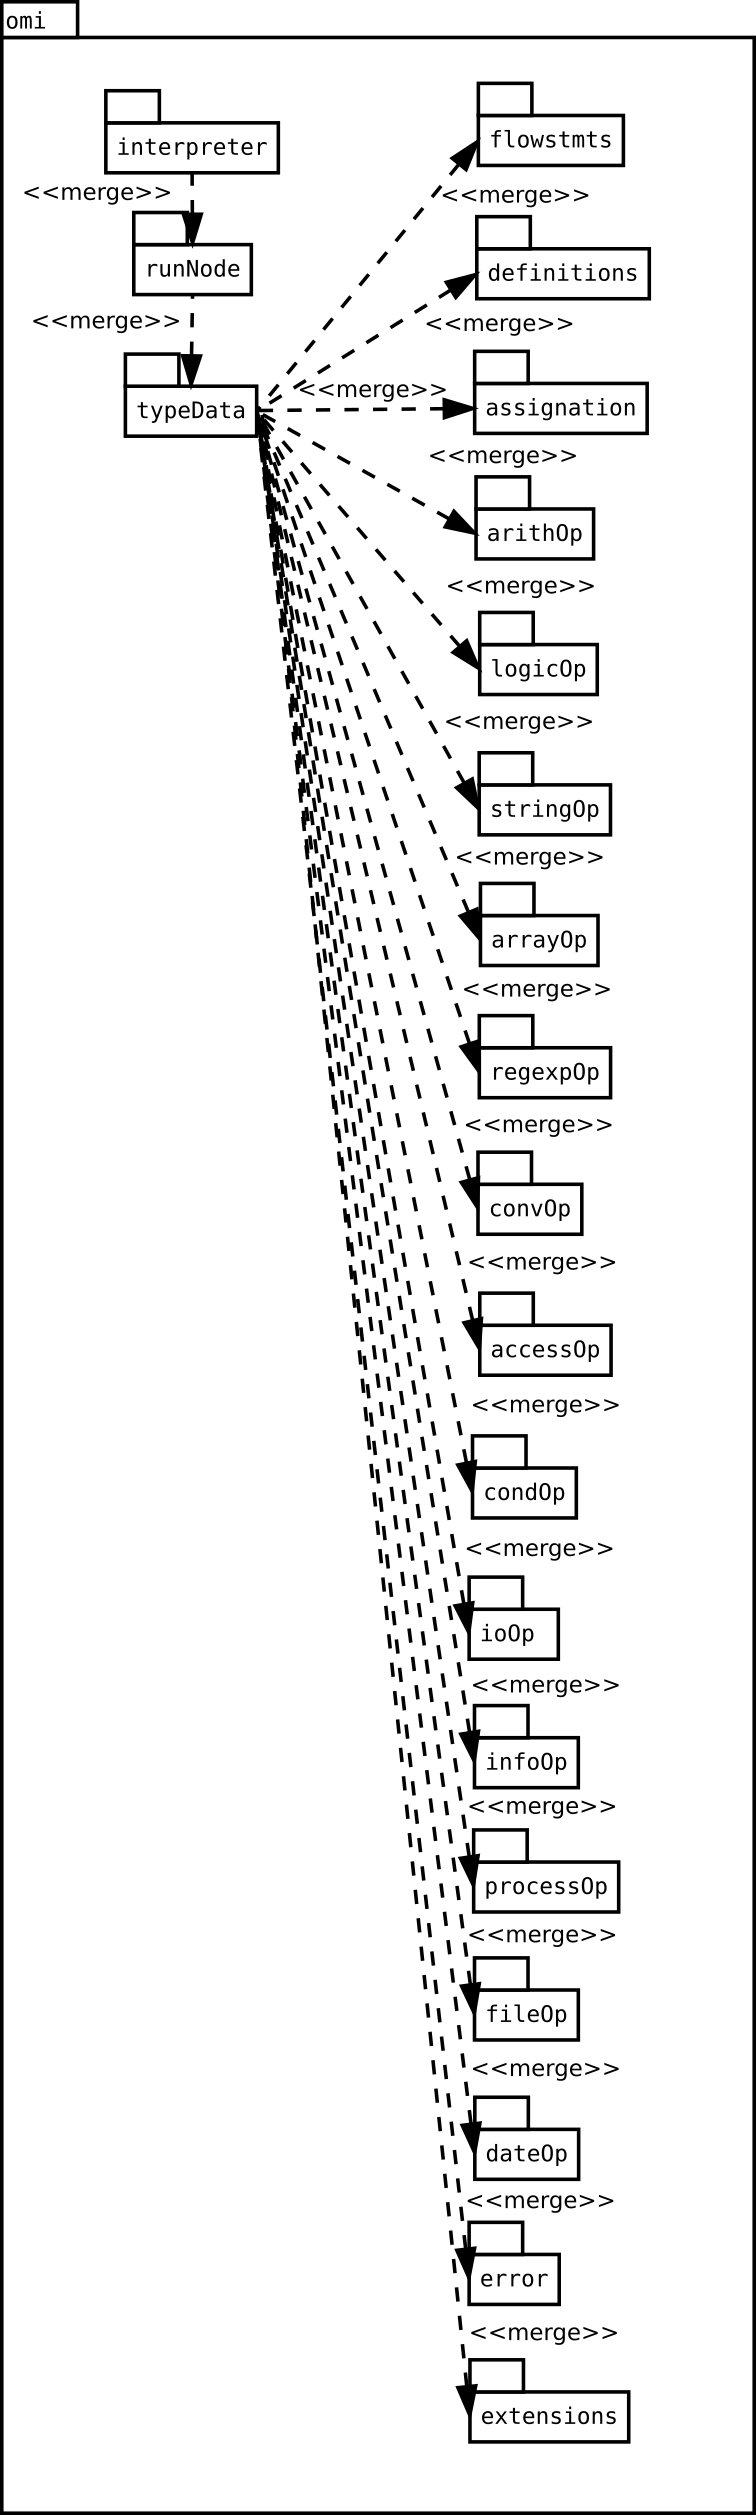
\includegraphics[scale=0.3]{package-omi.png} \\
%~ \end{center}
% ======================================================================
\subsection{Intérprete}
\begin{center}
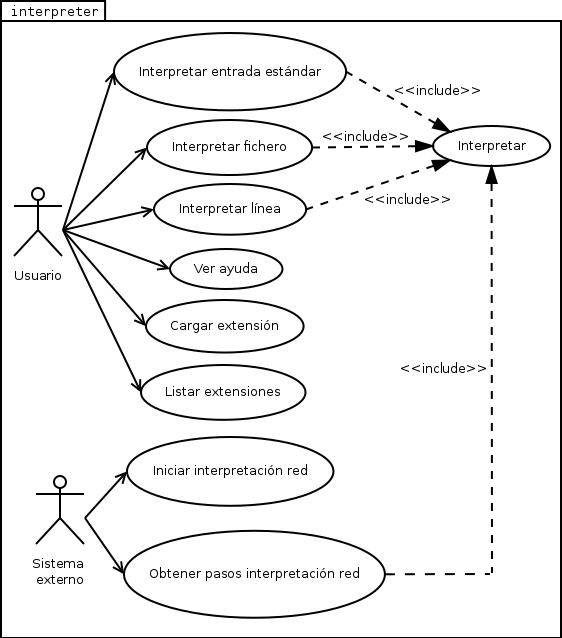
\includegraphics[scale=0.5]{use_case_interpreter.png} \\
\end{center}
% ----------------------------------------------------------------------
\subsubsection{Interpretar entrada estándar}

\begin{description}
  \item[Caso de Uso:] 
  Interpretar entrada estándar.
  \item[Tipo:] General.
  \item[Descripción:] 
  El usuario introduce un bloque de código en forma de cadena de 
  caracteres mediante la entrada estándar. El sistema lo interpreta 
  y ejecuta.
  \item[Actores:] 
  Usuario.
  \item[Precondiciones:] 
  El sistema debe estar esperando un bloque de código mediante la entrada estándar.
  \item[Postcondiciones:] 
  El código introducido es interpretado y ejecutado.
  \item[Escenario principal:] \hfill 
  \begin{enumerate}
   \item El usuario inicia el sistema facilitando un listado de argumentos.
   \item El sistema asigna como variables cada argumento y solicita contenido fuente al usuario. 
   \item El usuario introduce un bloque de código en la entrada estándar.
   \item El sistema obtiene el bloque de código a interpretar mediante la entrada estándar.
   \item Incluir (Interpretar). 
  \end{enumerate}
\end{description}
% ----------------------------------------------------------------------
\subsubsection{Interpretar fichero}

\begin{description}
   \item[Caso de Uso:]  Interpretar fichero.
   \item[Tipo:] General.
   \item[Descripción:] 
   El usuario indica un fichero que contiene código y que será 
   interpretado y ejecutado por el sistema.
   \item[Actores:] 
   Usuario.
   \item[Precondiciones:] 
   El sistema espera que se le indique un fichero.
   \item[Postcondiciones:] 
   El fichero es leído y el código en el mismo es interpretado y ejecutado.
   \item[Escenario principal:] \hfill
   \begin{enumerate}
   \item El usuario indica la ruta a un fichero y una serie de argumentos
   \item El sistema lee el fichero y obtiene el código en el mismo, además asigna cada argumento a variables.
   \item Incluir (Interpretar).
   \end{enumerate}
   
   \item[Flujo alternativo:] \hfill 
   \begin{enumerate} \itemsep1pt \parskip0pt \parsep0pt
   \setcounter{enumi}{1}
   \renewcommand{\labelenumi}{}
   \renewcommand{\labelenumiii}{\arabic{enumiii}.}
   \renewcommand{\labelenumii}{\arabic{enumi}\alph{enumii}.}
      \item 
      \begin {enumerate}
         \setcounter{enumii}{0}
         \item El fichero indicado no se encuentra.
         \begin{enumerate}
         \item El sistema informa del error y finaliza.
         \end{enumerate}
      \end{enumerate}
   \end{enumerate}
\end{description}

% ----------------------------------------------------------------------
\subsubsection{Interpretar línea}

\begin{description}
   \item[Caso de Uso:]  Interpretar línea.
   \item[Tipo:] General.
   \item[Descripción:] 
   El usuario introduce bloques de códigos denominados líneas
   de una forma interactiva. El sistema solicita por la entrada 
   estándar las líneas de código, que serán interpretadas y ejecutadas.
   \item[Actores:] 
   Usuario.
   \item[Precondiciones:] 
   El sistema se encuentra en modo interactivo.
   \item[Postcondiciones:] 
   Se interpreta cada línea introducida por el usuario
   \item[Escenario principal:] \hfill
   \begin{enumerate}
   \item El usuario inicia el sistema facilitando un listado de argumentos y la opción de interprete de línea.
   \item El sistema asigna como variables cada argumento y muestra un prompt que indica que espera una línea de código.
   \item El usuario introduce una línea de código.
   \item El sistema lee de la entrada estándar la línea introducida.
   \item Include (Interpretar). \\\\\hfill\hfill
   El sistema repite el caso de uso hasta que se interpreta una sentencia que produzca 
   la salida.
   \end{enumerate}
\end{description}

% ----------------------------------------------------------------------
\subsubsection{Interpretar}

\begin{description}
   \item[Caso de Uso:]  Interpretar.
   \item[Tipo:] General.
   \item[Nivel:]  Subfunción.
   \item[Descripción:] 
   El sistema analiza, interpreta y ejecuta un bloque de código facilitado por el usuario.
   Para ello comprueba que este cumple con el léxico y la gramática del lenguaje 
   que define, dividiéndolo a su vez en sentencias que serán interpretadas. 
   \item[Precondiciones:] 
   Se dispone de un bloque de código.
   \item[Postcondiciones:] 
   El bloque de código es interpretado.
   %~ \item [Puntos de extensión:] \hfill
   %~ \begin{description}
      %~ \item[Sentencia:] Según el tipo de sentencia.
   %~ \end{description}
   \item[Escenario principal:] \hfill
   \begin{enumerate}
   \item El sistema procesa y comprueba el bloque de código, aplicando
   la gramática y léxico que define.
   \item El sistema obtiene e interpreta cada sentencia en el código, produciéndose
   el significado semántico que estas encierran.
   \end{enumerate}
   \item[Flujo alternativo:] \hfill 
   \begin{enumerate} \itemsep1pt \parskip0pt \parsep0pt
   \setcounter{enumi}{0}
   \renewcommand{\labelenumi}{}
   \renewcommand{\labelenumiii}{\arabic{enumiii}.}
   \renewcommand{\labelenumii}{\arabic{enumi}\alph{enumii}.}
      \item 
      \begin {enumerate}
         \setcounter{enumii}{0}
         \item El código no respeta el léxico del lenguaje.
         \begin{enumerate}
         \item El sistema informa del error y finaliza.
         \end{enumerate}
      \end{enumerate}
   \end{enumerate}
   \begin{enumerate} \itemsep1pt \parskip0pt \parsep0pt
   \setcounter{enumi}{0}
   \renewcommand{\labelenumi}{}
   \renewcommand{\labelenumiii}{\arabic{enumiii}.}
   \renewcommand{\labelenumii}{\arabic{enumi}\alph{enumii}.}
      \item 
      \begin {enumerate}
         \setcounter{enumii}{1}
         \item El código no respeta la gramática del lenguaje.
         \begin{enumerate}
         \item El sistema informa del error y finaliza.
         \end{enumerate}
      \end{enumerate}
   \end{enumerate}
   \begin{enumerate} \itemsep1pt \parskip0pt \parsep0pt
   \setcounter{enumi}{1}
   \renewcommand{\labelenumi}{}
   \renewcommand{\labelenumiii}{\arabic{enumiii}.}
   \renewcommand{\labelenumii}{\arabic{enumi}\alph{enumii}.}
      \item 
      \begin {enumerate}
         \setcounter{enumii}{0}
         \item El código no contiene ninguna sentencia.
         \begin{enumerate}
         \item El sistema finaliza.
         \end{enumerate}
      \end{enumerate}
   \end{enumerate}
\end{description}

% ----------------------------------------------------------------------
\subsubsection{Ver ayuda}

\begin{description}
   \item[Caso de Uso:]  Ver ayuda.
   \item[Tipo:] General.
   \item[Descripción:] 
   Se muestra una ayuda que detalla cada opción disponible en el sistema.
   \item[Actores:] 
   Usuario.
   \item[Precondiciones:] 
   Sin precondiciones.
   \item[Postcondiciones:] 
   El sistema muestra un listado que presenta las distintas opciones.
   \item[Escenario principal:] \hfill
   \begin{enumerate}
   \item El usuario indica que quiere visualizar la ayuda.
   \item El sistema muestra un listado completo de las opciones que
   presenta. 
   \end{enumerate}
\end{description}

% ----------------------------------------------------------------------
\subsubsection{Cargar extensión}

\begin{description}
   \item[Caso de Uso:]  Cargar extensión.
   \item[Tipo:] General.
   \item[Descripción:] 
   El usuario indica que una extensión que será cargada por
   el sistema.
   \item[Actores:] 
   Usuario.
   \item[Precondiciones:] 
   Sin precondiciones.
   \item[Postcondiciones:] 
   El sistema cargar la extensión facilitada.
   \item[Escenario principal:] \hfill
   \begin{enumerate}
   \item El usuario indica la ruta a la extensión que desea cargar.
   \item El sistema carga la extensión para disponer de las distintas opciones que 
   ofrece. 
   \end{enumerate}
   \item[Flujo alternativo:] \hfill 
   \begin{enumerate} \itemsep1pt \parskip0pt \parsep0pt
   \setcounter{enumi}{1}
   \renewcommand{\labelenumi}{}
   \renewcommand{\labelenumiii}{\arabic{enumiii}.}
   \renewcommand{\labelenumii}{\arabic{enumi}\alph{enumii}.}
      \item 
      \begin {enumerate}
         \setcounter{enumii}{0}
         \item La extensión indicada no se encuentra.
         \begin{enumerate}
         \item El sistema informa del error.
         \end{enumerate}
      \end{enumerate}
   \end{enumerate}
   \begin{enumerate} \itemsep1pt \parskip0pt \parsep0pt
   \setcounter{enumi}{1}
   \renewcommand{\labelenumi}{}
   \renewcommand{\labelenumiii}{\arabic{enumiii}.}
   \renewcommand{\labelenumii}{\arabic{enumi}\alph{enumii}.}
      \item 
      \begin {enumerate}
         \setcounter{enumii}{1}
         \item La extensión indicada no es una extensión válida.
         \begin{enumerate}
         \item El sistema informa del error.
         \end{enumerate}
      \end{enumerate}
   \end{enumerate}
\end{description}

% ----------------------------------------------------------------------
\subsubsection{Listar extensiones}

\begin{description}
   \item[Caso de Uso:]  Listar extensiones.
   \item[Tipo:] General.
   \item[Descripción:] 
   Lista las extensiones que serán cargadas en cada ejecución del sistema.
   \item[Actores:] 
   Usuario.
   \item[Precondiciones:] 
   Sin precondiciones.
   \item[Postcondiciones:] 
   El sistema lista las extensiones que serán cargadas.
   \item[Escenario principal:] \hfill
   \begin{enumerate}
   \item El usuario indica que desea listar las extensiones cargadas.
   \item El sistema lista las extensiones cargadas por defecto. 
   \end{enumerate}
\end{description}

% ----------------------------------------------------------------------

%~ % ======================================================================
%~ 
%~ \pagebreak
%~ \subsection {Expresiones}
%~ \begin{center}
%~ 
\includegraphics[scale=0.5]{exp.png} \\
%~ \end{center}
%~ % ----------------------------------------------------------------------
%~ 
%~ \begin{framed}
%~ \FloatBarrier
%~ \begin{description}
   %~ \item[Caso de Uso:]  Expresión.
   %~ \item[Tipo:] General.
   %~ \item[Nivel:]  Subfunción.
   %~ \item[Descripción:] 
   %~ El sistema valora la expresión según la prioridad de operadores
   %~ que define. 
   %~ \item[Precondiciones:] 
   %~ La expresión cumple con el léxico y gramática del lenguaje.
   %~ \item[Postcondiciones:] 
   %~ El sistema interpreta la expresión obteniendo su valor asociado.
   %~ \item[Puntos de extensión:] \hfill
      %~ \begin{description}
         %~ \item [Valorar:] Según tipo de operador o subexpresión
      %~ \end{description}
   %~ \item[Escenario principal:] \hfill
   %~ \begin{enumerate}
   %~ \item El sistema determina el operador 
   %~ o subexpresión de mayor prioridad.
   %~ \item Valorar: punto de extensión 
   %~ \end{enumerate}
%~ \end{description}
 %~ \FloatBarrier
%~ \end{framed}
%~ % ----------------------------------------------------------------------
%~ % ======================================================================
%~ 
%~ 
%~ \subsection {Tipos de datos}
%~ \begin{center}
%~ 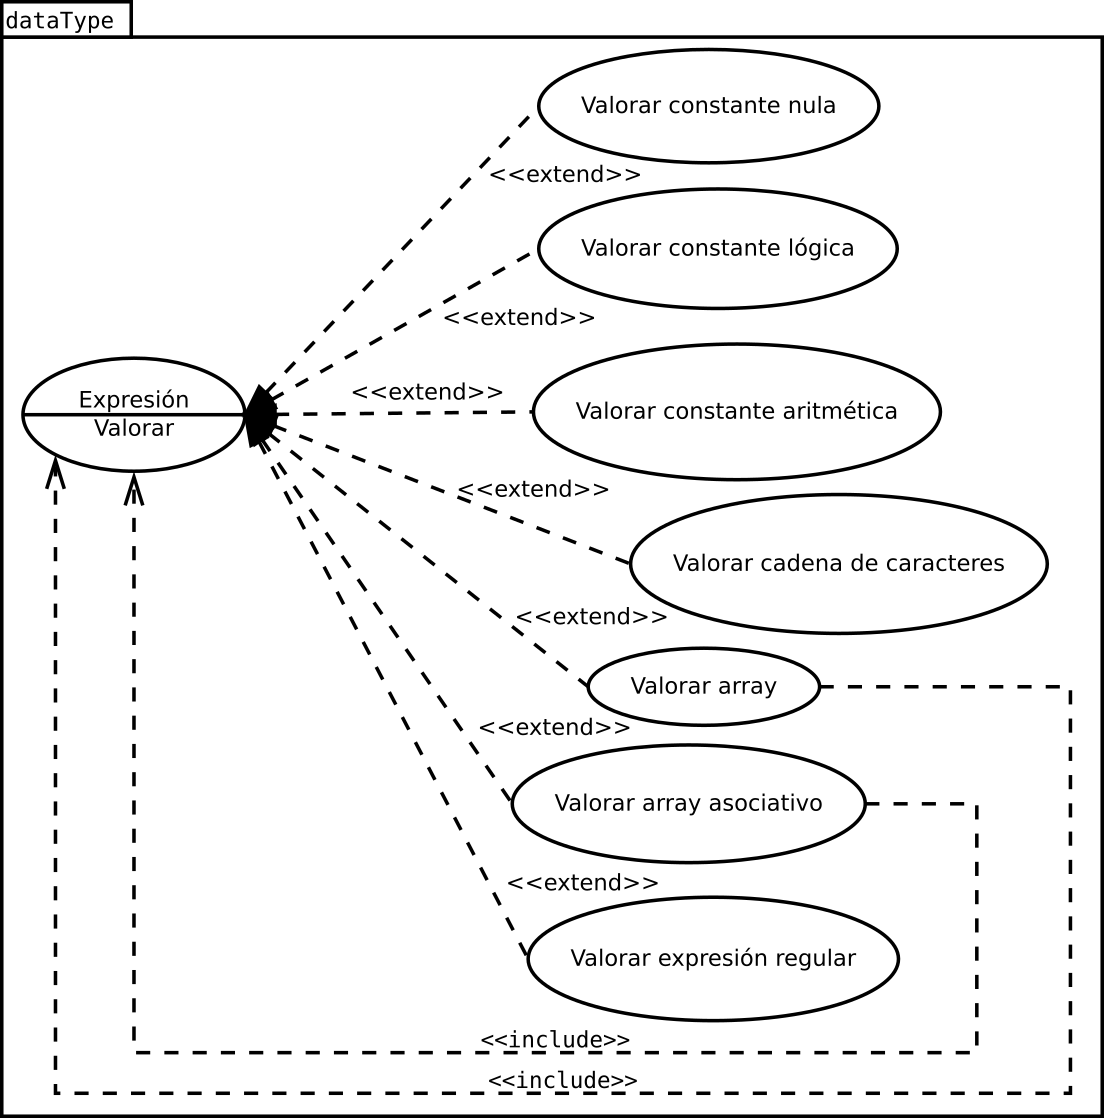
\includegraphics[scale=0.4]{dataType.png} \\
%~ \end{center}
%~ % ----------------------------------------------------------------------
%~ \subsubsection{Valorar constante nula}
%~ \begin{framed}
%~ \FloatBarrier
%~ \begin{description}
   %~ \item[Caso de Uso:] Valorar constante nula.
   %~ \item [Tipo:] Expresión.
   %~ \item[Nivel:]  Subfunción.
   %~ \item[Descripción:] 
   %~ El sistema valora una expresión o subexpresión correspondiente a
   %~ la constante nula codificada de forma explicita.
   %~ \item[Precondiciones:] 
   %~ El sistema se encuentra valorando una expresión y esta es un valor constante nulo.
   %~ \item[Postcondiciones:] 
   %~ El sistema atribuye nulo como valor de la expresión.
   %~ \item[Escenario principal:] \hfill
   %~ \begin{enumerate}
   %~ \item El sistema otorga a la expresión en valor nulo.
   %~ \end{enumerate}
%~ \end{description}
 %~ \FloatBarrier
%~ \end{framed}
%~ 
%~ \subsubsection{Valorar constante lógica}
%~ \begin{framed}
%~ \FloatBarrier
%~ \begin{description}
   %~ \item[Caso de Uso:]  Valorar constante lógica.
   %~ \item [Tipo:] Expresión.
   %~ \item[Nivel:]  Subfunción.
   %~ \item[Descripción:] 
   %~ El sistema valora una expresión o subexpresión correspondiente
   %~ a una constante lógica verdadero o falso.
   %~ \item[Precondiciones:] 
   %~ El sistema se encuentra valorando una expresión y esta es una constante lógica.
   %~ \item[Postcondiciones:] 
   %~ El sistema atribuye verdadero o falso como valor de la expresión.
   %~ \item[Escenario principal:] \hfill
   %~ \begin{enumerate}
   %~ \item El sistema otorga a la expresión el valor lógico verdadero 
   %~ si se corresponde con la expresión ``true'' o falso si se corresponde 
   %~ con ``false''.
   %~ \end{enumerate}
%~ \end{description}
 %~ \FloatBarrier
%~ \end{framed}
%~ 
%~ \subsubsection{Valorar constante aritmética}
%~ \begin{framed}
%~ \FloatBarrier
%~ \begin{description}
   %~ \item[Caso de Uso:]  Valorar constante aritmética.
   %~ \item [Tipo:] Expresión.
   %~ \item[Nivel:]  Subfunción.
   %~ \item[Descripción:] 
   %~ El sistema valora una expresión o subexpresión que se corresponde con
   %~ un número dentro del conjunto de los racionales.
   %~ \item[Precondiciones:] 
   %~ El sistema se encuentra valorando una expresión y esta es una constante numérica.
   %~ \item[Postcondiciones:] 
   %~ El sistema atribuye el número como valor de la expresión.
   %~ \item[Escenario principal:] \hfill
   %~ \begin{enumerate}
   %~ \item El sistema otorga a la expresión el valor numérico codificado 
   %~ en la misma.
   %~ \end{enumerate}
%~ \end{description}
 %~ \FloatBarrier
%~ \end{framed}
%~ 
%~ \subsubsection {Valorar cadena de caracteres}
%~ \begin{framed}
%~ \FloatBarrier
%~ \begin{description}
   %~ \item[Caso de Uso:]  Valorar cadena de caracteres.
   %~ \item [Tipo:] Expresión.
   %~ \item[Nivel:]  Subfunción.
   %~ \item[Descripción:] 
   %~ El sistema valora una expresión o subexpresión correspondiente a
   %~ una cadena de caracteres constante.
   %~ \item[Precondiciones:] 
   %~ El sistema se encuentra valorando una expresión y esta es un valor cadena de caracteres.
   %~ \item[Postcondiciones:] 
   %~ El sistema atribuye la cadena de caracteres como valor de la expresión.
   %~ \item[Escenario principal:] \hfill
   %~ \begin{enumerate}
   %~ \item El sistema otorga a la expresión el valor correspondiente a la cadena codificada
   %~ en la misma.
   %~ \end{enumerate}
%~ \end{description}
 %~ \FloatBarrier
%~ \end{framed}
%~ \subsubsection {Valorar array}
%~ \begin{framed}
%~ \FloatBarrier
%~ \begin{description}
   %~ \item[Caso de Uso:]  Valorar array.
   %~ \item [Tipo:] Expresión.
   %~ \item[Nivel:]  Subfunción.
   %~ \item[Descripción:] 
   %~ El sistema valora una expresión o subexpresión correspondiente a
   %~ un array no asociativo.
   %~ \item[Precondiciones:] 
   %~ El sistema se encuentra valorando una expresión y esta es un array.
   %~ \item[Postcondiciones:] 
   %~ El sistema atribuye el array como valor de la expresión.
   %~ \item[Escenario principal:] \hfill
   %~ \begin{enumerate}
   %~ \item El sistema obtiene la subexpresión correspondiente al primer elemento.
   %~ \item Include (Expresión)
   %~ \item Atribuye el valor de la subexpresión como último elemento en el array.\\\\\hfill\hfill
   %~ Se repiten los pasos 2-3 secuencialmente para cada elemento.
   %~ \end{enumerate}
   %~ \item[Flujo alternativo:] \hfill 
   %~ \begin{enumerate} \itemsep1pt \parskip0pt \parsep0pt
   %~ \setcounter{enumi}{0}
   %~ \renewcommand{\labelenumi}{}
   %~ \renewcommand{\labelenumiii}{\arabic{enumiii}.}
   %~ \renewcommand{\labelenumii}{\arabic{enumi}\alph{enumii}.}
      %~ \item 
      %~ \begin {enumerate}
         %~ \setcounter{enumii}{0}
         %~ \item El array no contiene elementos.
         %~ \begin{enumerate}
         %~ \item El sistema atribuye como valor de la expresión el array vacío.
         %~ \end{enumerate}
      %~ \end{enumerate}
   %~ \end{enumerate}
%~ \end{description}
 %~ \FloatBarrier
%~ \end{framed}
%~ \subsubsection {Valorar array asociativo}
%~ \begin{framed}
%~ \FloatBarrier
%~ \begin{description}
   %~ \item[Caso de Uso:]  Array asociativo.
   %~ \item [Tipo:] Expresión.
   %~ \item[Nivel:]  Subfunción.
   %~ \item[Descripción:] 
   %~ El sistema valora una expresión o subexpresión correspondiente a
   %~ un array asociativo .
   %~ \item[Precondiciones:] 
   %~ El sistema se encuentra valorando una expresión y esta es un valor array asociativo.
   %~ \item[Postcondiciones:] 
   %~ El sistema atribuye el array asociativo como valor de la expresión.
   %~ \item[Escenario principal:] \hfill
   %~ \begin{enumerate}
   %~ \item El sistema obtiene la subexpresión correspondiente al primer elemento.
   %~ \item El sistema obtiene la subexpresión correspondiente la clave.
   %~ \item Include (Expresión)
   %~ \item El sistema obtiene la subexpresión correspondiente al valor.
   %~ \item Include (Expresión)
   %~ \item Atribuye el par clave/valor como último elemento en el array.\\\\\hfill\hfill
   %~ Se repiten los pasos 2-6 secuencialmente para cada elemento.
   %~ \end{enumerate}
    %~ \item[Flujo alternativo:] \hfill 
   %~ \begin{enumerate} \itemsep1pt \parskip0pt \parsep0pt
   %~ \setcounter{enumi}{0}
   %~ \renewcommand{\labelenumi}{}
   %~ \renewcommand{\labelenumiii}{\arabic{enumiii}.}
   %~ \renewcommand{\labelenumii}{\arabic{enumi}\alph{enumii}.}
      %~ \item 
      %~ \begin {enumerate}
         %~ \setcounter{enumii}{0}
         %~ \item El array no contiene elementos.
         %~ \begin{enumerate}
         %~ \item El sistema atribuye como valor de la expresión el array vacío.
         %~ \end{enumerate}
      %~ \end{enumerate}
   %~ \end{enumerate}
%~ \end{description}
 %~ \FloatBarrier
%~ \end{framed}
%~ \subsubsection {Valorar expresión regular}
%~ \begin{framed}
%~ \FloatBarrier
%~ \begin{description}
   %~ \item[Caso de Uso:]  Valor expresión regular.
   %~ \item [Tipo:] Expresión.
   %~ \item[Nivel:]  Subfunción.
   %~ \item[Descripción:] 
   %~ El sistema valora una expresión o subexpresión correspondiente a
   %~ una expresión regular PERL.
   %~ \item[Precondiciones:] 
   %~ El sistema se encuentra valorando una expresión y esta es una expresión regular PERL.
   %~ \item[Postcondiciones:] 
   %~ El sistema atribuye la expresión regular como valor de la expresión PERL.
   %~ \item[Escenario principal:] \hfill
   %~ \begin{enumerate}
   %~ \item El sistema obtiene la expresión regular codificada.
   %~ \item El sistema atribuye la expresión regular como valor de la expresión
   %~ \end{enumerate}
    %~ \item[Flujo alternativo:] \hfill 
   %~ \begin{enumerate} \itemsep1pt \parskip0pt \parsep0pt
   %~ \setcounter{enumi}{0}
   %~ \renewcommand{\labelenumi}{}
   %~ \renewcommand{\labelenumiii}{\arabic{enumiii}.}
   %~ \renewcommand{\labelenumii}{\arabic{enumi}\alph{enumii}.}
      %~ \item 
      %~ \begin {enumerate}
         %~ \setcounter{enumii}{0}
         %~ \item La expresión regular no mantiene una sintaxis PERL.
         %~ \begin{enumerate}
         %~ \item El sistema informa del error y finaliza la interpretación
         %~ de la sentencia correspondiente.
         %~ \end{enumerate}
      %~ \end{enumerate}
   %~ \end{enumerate}
%~ \end{description}
 %~ \FloatBarrier
%~ \end{framed}
%~ 
%~ % ----------------------------------------------------------------------
%~ % ======================================================================
%~ 
%~ 
%~ \subsection {Sentencias de control de flujo}
%~ \begin{center}
%~ 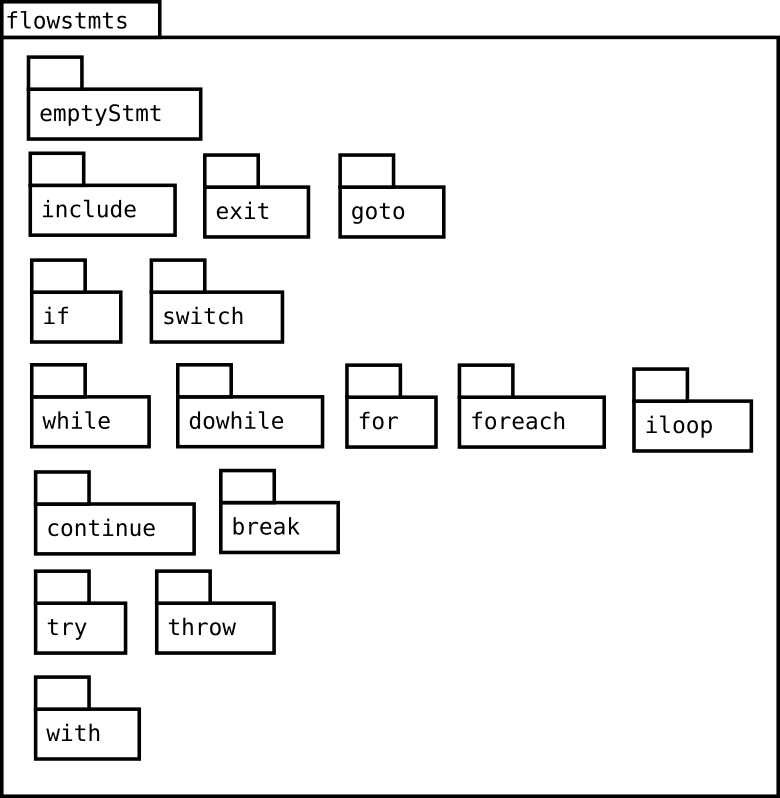
\includegraphics[scale=0.4]{flowstmts.png} \\
%~ \end{center}
%~ % ----------------------------------------------------------------------
%~ \subsubsection {Sentencia vacía}
%~ \begin{center}
%~ 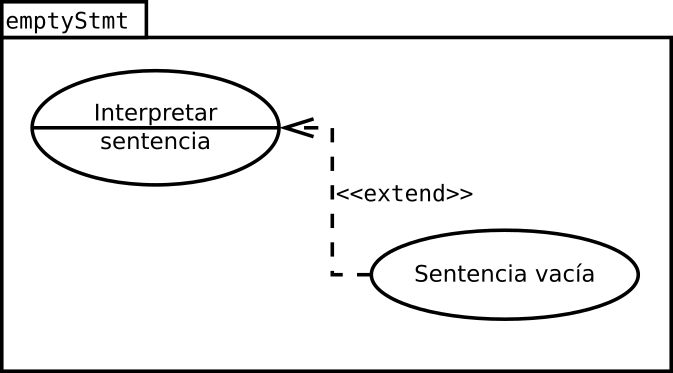
\includegraphics[scale=0.4]{emptyStmt.png} \\
%~ \end{center}
%~ \begin{framed}
%~ \FloatBarrier
%~ \begin{description}
   %~ \item[Caso de Uso:]  Sentencia vacía.
   %~ \item [Tipo:] Sentencia.
   %~ \item[Nivel:]  Subfunción.
   %~ \item[Descripción:] 
   %~ Se interpreta una sentencia vacía sin producir resultado alguno.
   %~ \item[Precondiciones:] 
   %~ La sentencia interpretada es una sentencia vacía.
   %~ \item[Postcondiciones:] No tiene.
   %~ \item[Escenario principal:] \hfill
   %~ \begin{enumerate}
   %~ \item El sistema no realiza ninguna acción.
   %~ \end{enumerate}
%~ \end{description}
 %~ \FloatBarrier
%~ \end{framed}
%~ % ----------------------------------------------------------------------
%~ \subsubsection {Sentencia include}
%~ \begin{center}
%~ 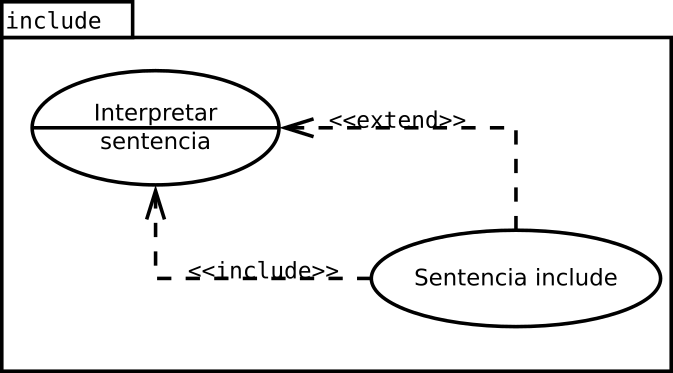
\includegraphics[scale=0.4]{include.png} \\
%~ \end{center}
%~ \begin{framed}
%~ \FloatBarrier
%~ \begin{description}
   %~ \item[Caso de Uso:]  Sentencia include.
   %~ \item [Tipo:] Sentencia.
   %~ \item[Nivel:]  Subfunción.
   %~ \item[Descripción:] 
   %~ Se interpreta una sentencia include, lo que 
   %~ se corresponde con la lectura e interpretación del fichero codificado 
   %~ en la misma. 
   %~ \item[Precondiciones:] 
   %~ La sentencia interpretada es una sentencia include.
   %~ \item[Postcondiciones:] El fichero es leído e interpretado
   %~ \item[Escenario principal:] \hfill
   %~ \begin{enumerate}
   %~ \item El sistema obtiene el código fuente del fichero.
   %~ \item Include (Interpretar).
   %~ \end{enumerate}
   %~ \item[Flujo alternativo:] \hfill 
   %~ \begin{enumerate} \itemsep1pt \parskip0pt \parsep0pt
   %~ \setcounter{enumi}{0}
   %~ \renewcommand{\labelenumi}{}
   %~ \renewcommand{\labelenumiii}{\arabic{enumiii}.}
   %~ \renewcommand{\labelenumii}{\arabic{enumi}\alph{enumii}.}
      %~ \item 
      %~ \begin {enumerate}
         %~ \setcounter{enumii}{0}
         %~ \item El fichero no existe.
         %~ \begin{enumerate}
         %~ \item El sistema informa del error y finaliza la  interpretación 
         %~ de la sentencia actual.
         %~ \end{enumerate}
      %~ \end{enumerate}
   %~ \end{enumerate}
%~ \end{description}
 %~ \FloatBarrier
%~ \end{framed}
%~ % ----------------------------------------------------------------------
%~ 
%~ \subsubsection {Sentencia exit}
%~ \begin{center}
%~ 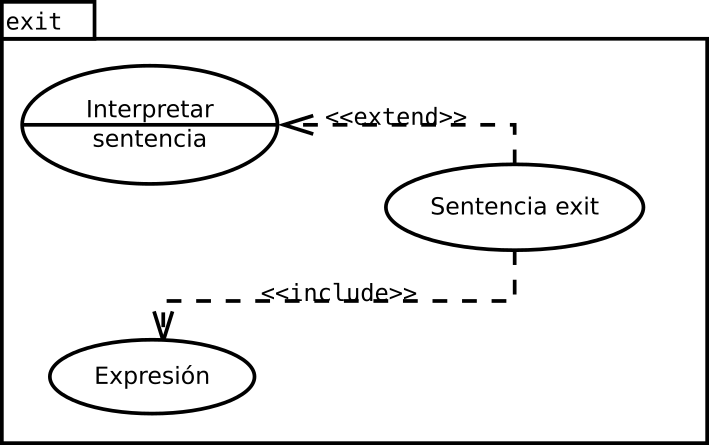
\includegraphics[scale=0.4]{exit.png} \\
%~ \end{center}
%~ \begin{framed}
%~ \FloatBarrier
%~ \begin{description}
   %~ \item[Caso de Uso:]  Sentencia exit.
   %~ \item [Tipo:] Sentencia.
   %~ \item[Nivel:]  Subfunción.
   %~ \item[Descripción:] 
   %~ Se interpreta una sentencia exit, lo que 
   %~ se corresponde con la salida y finalización del sistema. 
   %~ \item[Precondiciones:] 
   %~ La sentencia interpretada es una sentencia exit.
   %~ \item[Postcondiciones:] Se sale del sistema con el código codificado
   %~ en la sentencia.
   %~ \item[Escenario principal:] \hfill
   %~ \begin{enumerate}
   %~ \item El sistema obtiene la expresión correspondiente al código de salida.
   %~ \item Include (Expresión)
   %~ \item El sistema finaliza su ejecución devolviendo el valor del código.
   %~ \end{enumerate}
%~ \end{description}
 %~ \FloatBarrier
%~ \end{framed}
%~ % ----------------------------------------------------------------------
%~ \subsubsection {Sentencia goto}
%~ \begin{center}
%~ 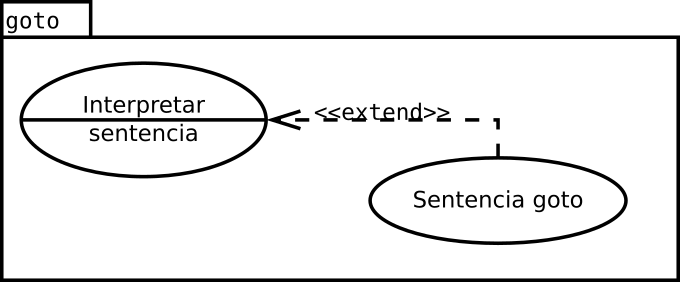
\includegraphics[scale=0.4]{goto.png} \\
%~ \end{center}
%~ \begin{framed}
%~ \FloatBarrier
%~ \begin{description}
   %~ \item[Caso de Uso:]  Sentencia goto.
   %~ \item [Tipo:] Sentencia.
   %~ \item[Nivel:]  Subfunción.
   %~ \item[Descripción:] 
   %~ Hace que la siguiente sentencia interpretada sea la que esté referenciada 
   %~ por la etiqueta codificada en la sentencia. 
   %~ \item[Precondiciones:] 
   %~ La sentencia interpretada es una sentencia goto.
   %~ \item[Postcondiciones:] La siguiente sentencia que se ejecutará se 
   %~ corresponde con la referenciada por la etiqueta indicada.
   %~ \item[Escenario principal:] \hfill
   %~ \begin{enumerate}
   %~ \item El sistema obtiene la etiqueta codificada en la sentencia.
   %~ \item El sistema cambia el flujo de ejecución a la sentencia obtenida.
   %~ \end{enumerate}
   %~ \item[Flujo alternativo:] \hfill 
   %~ \begin{enumerate} \itemsep1pt \parskip0pt \parsep0pt
   %~ \setcounter{enumi}{0}
   %~ \renewcommand{\labelenumi}{}
   %~ \renewcommand{\labelenumiii}{\arabic{enumiii}.}
   %~ \renewcommand{\labelenumii}{\arabic{enumi}\alph{enumii}.}
      %~ \item 
      %~ \begin {enumerate}
         %~ \setcounter{enumii}{0}
         %~ \item No existe definida la etiqueta codificada.
         %~ \begin{enumerate}
         %~ \item El sistema informa del error y finaliza la  interpretación 
         %~ de la sentencia actual.
         %~ \end{enumerate}
      %~ \end{enumerate}
   %~ \end{enumerate}
%~ \end{description}
 %~ \FloatBarrier
%~ \end{framed}
%~ % ----------------------------------------------------------------------
%~ \subsubsection {Sentencia if}
%~ \begin{center}
%~ 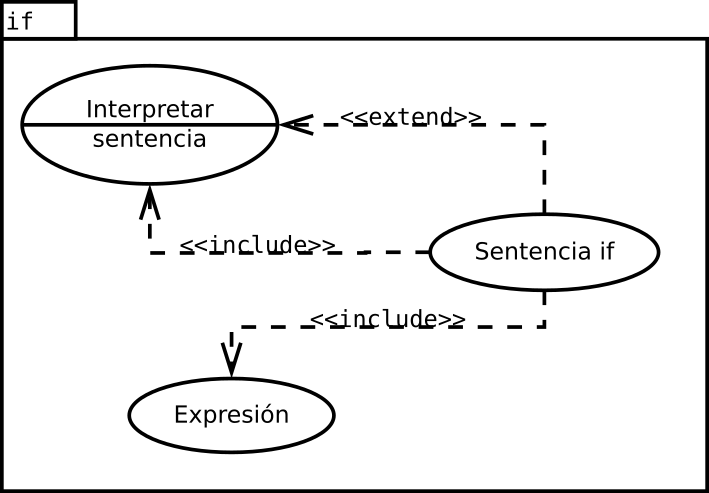
\includegraphics[scale=0.4]{if.png} \\
%~ \end{center}
%~ \begin{framed}
%~ \FloatBarrier
%~ \begin{description}
   %~ \item[Caso de Uso:]  Sentencia if.
   %~ \item [Tipo:] Sentencia.
   %~ \item[Nivel:]  Subfunción.
   %~ \item[Descripción:] 
   %~ Interpreta una sentencia if, lo que implica que se interpretará el 
   %~ bloque de sentencias ``then'' si la expresión de condición es
   %~ verdadera o el bloque ``else'' si es falsa.
   %~ 
   %~ \item[Precondiciones:] 
   %~ La sentencia interpretada es una sentencia if.
   %~ \item[Postcondiciones:] 
   %~ La sentencia if queda interpretada.   
   %~ \item[Escenario principal:] \hfill
   %~ \begin{enumerate}
   %~ \item El sistema obtiene la expresión de condición.
   %~ \item Include (Expresión).
   %~ \item Si la expresión tiene valor lógico verdadero el sistema obtiene el bloque de sentencias ``then''.
   %~ \item Include (Interpretar).
   %~ \end{enumerate}
   %~ \item[Flujo alternativo:] \hfill 
   %~ \begin{enumerate} \itemsep1pt \parskip0pt \parsep0pt
   %~ \setcounter{enumi}{2}
   %~ \renewcommand{\labelenumi}{}
   %~ \renewcommand{\labelenumiii}{\arabic{enumiii}.}
   %~ \renewcommand{\labelenumii}{\arabic{enumi}\alph{enumii}.}
      %~ \item 
      %~ \begin {enumerate}
         %~ \setcounter{enumii}{0}
         %~ \item La expresión no tiene valor lógico asociado.
         %~ \begin{enumerate}
         %~ \item Esta es considerada falsa y se prosigue con el caso de uso.  
         %~ \end{enumerate}
      %~ \end{enumerate}
   %~ \end{enumerate}
   %~ \begin{enumerate} \itemsep1pt \parskip0pt \parsep0pt
   %~ \setcounter{enumi}{2}
   %~ \renewcommand{\labelenumi}{}
   %~ \renewcommand{\labelenumiii}{\arabic{enumiii}.}
   %~ \renewcommand{\labelenumii}{\arabic{enumi}\alph{enumii}.}
      %~ \item 
      %~ \begin {enumerate}
         %~ \setcounter{enumii}{1}
         %~ \item La expresión tiene valor falso y la sentencia codifica un bloque ``else''.
         %~ \begin{enumerate}
         %~ \item El sistema obtiene el bloque de sentencias ``else''.
         %~ \item Include (Interpretar) 
         %~ \end{enumerate}
      %~ \end{enumerate}
   %~ \end{enumerate}
   %~ \begin{enumerate} \itemsep1pt \parskip0pt \parsep0pt
   %~ \setcounter{enumi}{2}
   %~ \renewcommand{\labelenumi}{}
   %~ \renewcommand{\labelenumiii}{\arabic{enumiii}.}
   %~ \renewcommand{\labelenumii}{\arabic{enumi}\alph{enumii}.}
      %~ \item 
      %~ \begin {enumerate}
         %~ \setcounter{enumii}{2}
         %~ \item La expresión tiene valor falso y la sentencia no codifica un bloque ``else''.
         %~ \begin{enumerate}
         %~ \item El sistema no realiza ninguna acción. 
         %~ \end{enumerate}
      %~ \end{enumerate}
   %~ \end{enumerate}
%~ \end{description}
 %~ \FloatBarrier
%~ \end{framed}
%~ % ----------------------------------------------------------------------
%~ \subsubsection {Sentencia switch}
%~ \begin{center}
%~ 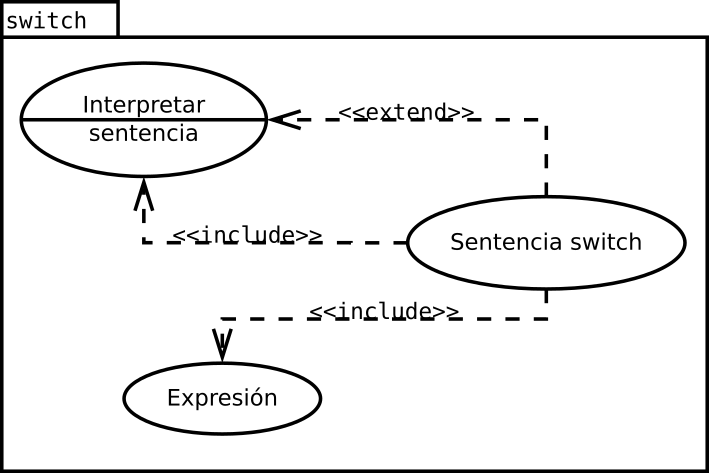
\includegraphics[scale=0.4]{switch.png} \\
%~ \end{center}
%~ \begin{framed}
%~ \FloatBarrier
%~ \begin{description}
   %~ \item[Caso de Uso:]  Sentencia switch.
   %~ \item [Tipo:] Sentencia. 
   %~ \item[Nivel:]  Subfunción.
   %~ \item[Descripción:] 
   %~ Interpreta una sentencia switch, por lo que se ejecutará el bloque de sentencias 
   %~ correspondiente según el valor de la expresión condición, y todos los bloques
   %~ siguientes.
   %~ \item[Precondiciones:] 
   %~ La sentencia interpretada es una sentencia switch.
   %~ \item[Postcondiciones:] 
       %~ La sentencia switch queda interpretada.
   %~ \item[Escenario principal:] \hfill
   %~ \begin{enumerate}
   %~ \item El sistema obtiene la expresión de condición.
   %~ \item Include (Expresión).
   %~ \item Se obtiene el bloque de sentencias correspondiente al valor de la expresión.
   %~ \item Include (Interpretar). \\\\ \hfill
      %~ Se repite el paso 4 por cada bloque de sentencias de los casos siguientes.
   %~ \end{enumerate}
   %~ \item[Flujo alternativo:] \hfill 
   %~ \begin{enumerate} \itemsep1pt \parskip0pt \parsep0pt
   %~ \setcounter{enumi}{2}
   %~ \renewcommand{\labelenumi}{}
   %~ \renewcommand{\labelenumiii}{\arabic{enumiii}.}
   %~ \renewcommand{\labelenumii}{\arabic{enumi}\alph{enumii}.}
      %~ \item 
      %~ \begin {enumerate}
         %~ \setcounter{enumii}{0}
         %~ \item No existe bloque de sentencias para el valor de la expresión, pero 
         %~ existe un bloque de sentencias por defecto.
         %~ \begin{enumerate}
         %~ \item Se obtiene el bloque de sentencias por defecto.
         %~ \item Include (Interpretar)  
         %~ \end{enumerate}
      %~ \end{enumerate}
   %~ \end{enumerate}
   %~ \begin{enumerate} \itemsep1pt \parskip0pt \parsep0pt
   %~ \setcounter{enumi}{2}
   %~ \renewcommand{\labelenumi}{}
   %~ \renewcommand{\labelenumiii}{\arabic{enumiii}.}
   %~ \renewcommand{\labelenumii}{\arabic{enumi}\alph{enumii}.}
      %~ \item 
      %~ \begin {enumerate}
         %~ \setcounter{enumii}{1}
         %~ \item No existe bloque de sentencias para el valor de la expresión y 
         %~ tampoco existe un bloque de sentencias por defecto.
         %~ \begin{enumerate}
         %~ \item El sistema no realiza ninguna acción.
         %~ \end{enumerate}
      %~ \end{enumerate}
   %~ \end{enumerate}
%~ \end{description}
 %~ \FloatBarrier
%~ \end{framed}
%~ % ----------------------------------------------------------------------
%~ \subsubsection {Sentencia while}
%~ \begin{center}
%~ 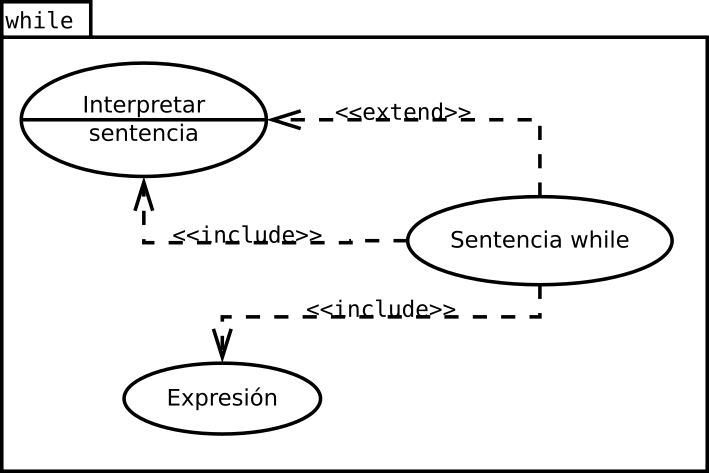
\includegraphics[scale=0.4]{while.png} \\
%~ \end{center}
%~ \begin{framed}
%~ \FloatBarrier
%~ \begin{description}
   %~ \item[Caso de Uso:]  Sentencia while.
   %~ \item [Tipo:] Sentencia.
   %~ \item[Nivel:]  Subfunción.
   %~ \item[Descripción:] 
   %~ Interpreta la sentencia while, lo que implica que se ejecutará el bloque 
   %~ de sentencias mientras el valor de la expresión de condición sea verdadera.
   %~ \item[Precondiciones:] 
   %~ La sentencia interpretada es una sentencia while.
   %~ \item[Postcondiciones:] 
   %~ La sentencia while queda interpretada.
   %~ \item[Escenario principal:] \hfill
   %~ \begin{enumerate}
   %~ \item El sistema obtiene la expresión de condición.
   %~ \item Include (Expresión).
   %~ \item Si la expresión es verdadera obtiene el bloque de sentencias.
   %~ \item Include (Interpretar). \\\\ \hfill
      %~ Se repite el paso 1-4 hasta que la expresión sea valorada como falsa.
   %~ \end{enumerate}
   %~ \item[Flujo alternativo:] \hfill 
   %~ \begin{enumerate} \itemsep1pt \parskip0pt \parsep0pt
   %~ \setcounter{enumi}{2}
   %~ \renewcommand{\labelenumi}{}
   %~ \renewcommand{\labelenumiii}{\arabic{enumiii}.}
   %~ \renewcommand{\labelenumii}{\arabic{enumi}\alph{enumii}.}
      %~ \item 
      %~ \begin {enumerate}
         %~ \setcounter{enumii}{0}
         %~ \item La expresión no tiene un valor booleano asociado.
         %~ \begin{enumerate}
         %~ \item Se considera como si tuviera valor falso y se continua con el caso de uso.
         %~ \end{enumerate}
      %~ \end{enumerate}
   %~ \end{enumerate}
%~ \end{description}
 %~ \FloatBarrier
%~ \end{framed}
%~ % ----------------------------------------------------------------------
%~ \subsubsection {Sentencia do...while}
%~ \begin{center}
%~ 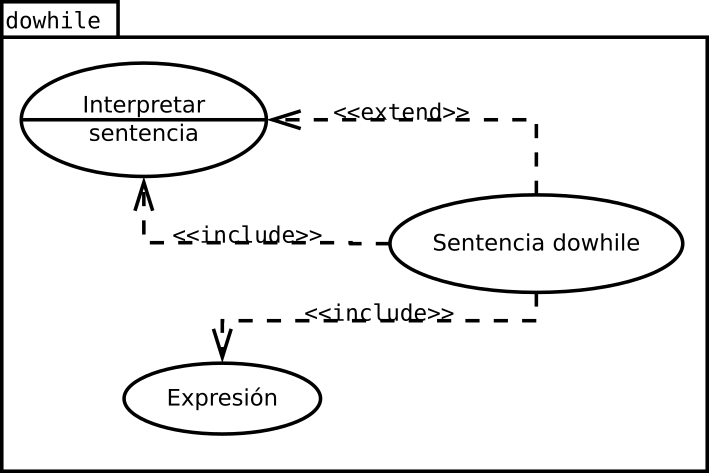
\includegraphics[scale=0.4]{dowhile.png} \\
%~ \end{center}
%~ \begin{framed}
%~ \FloatBarrier
%~ \begin{description}
   %~ \item[Caso de Uso:]  Sentencia do...while.
   %~ \item [Tipo:] Sentencia.
   %~ \item[Nivel:]  Subfunción.
   %~ \item[Descripción:] 
   %~ Interpreta una sentencia do...while, lo que implica que se ejecutará 
   %~ el bloque de sentencias, al menos una vez, y mientras el valor de la expresión
   %~ de condición sea verdadera.
   %~ \item[Precondiciones:] 
   %~ La sentencia interpretada es una sentencia do...while.
   %~ \item[Postcondiciones:] 
   %~ La sentencia do...while queda interpretada.
   %~ \item[Escenario principal:] \hfill
   %~ \begin{enumerate}
   %~ \item El sistema obtiene el bloque de sentencias.
   %~ \item Include (Interpretar). 
   %~ \item El sistema obtiene la expresión de condición.
   %~ \item Include (Expresión).\\\\ \hfill
      %~ Se repite el paso 1-4 hasta que la expresión sea valorada como falsa.
   %~ \end{enumerate}
   %~ \item[Flujo alternativo:] \hfill 
   %~ \begin{enumerate} \itemsep1pt \parskip0pt \parsep0pt
   %~ \setcounter{enumi}{3}
   %~ \renewcommand{\labelenumi}{}
   %~ \renewcommand{\labelenumiii}{\arabic{enumiii}.}
   %~ \renewcommand{\labelenumii}{\arabic{enumi}\alph{enumii}.}
      %~ \item 
      %~ \begin {enumerate}
         %~ \setcounter{enumii}{0}
         %~ \item La expresión no tiene un valor booleano asociado.
         %~ \begin{enumerate}
         %~ \item Se considera como si tuviera valor falso y se continua con el caso de uso.
         %~ \end{enumerate}
      %~ \end{enumerate}
   %~ \end{enumerate}
%~ \end{description}
 %~ \FloatBarrier
%~ \end{framed}
%~ % ----------------------------------------------------------------------
%~ \subsubsection {Sentencia for}
%~ \begin{center}
%~ 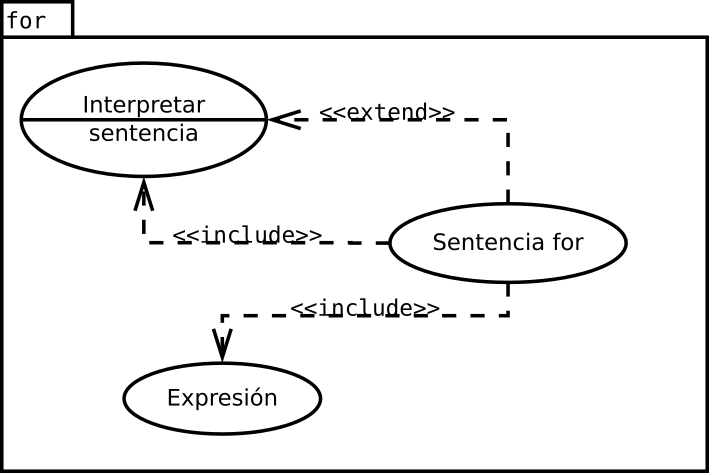
\includegraphics[scale=0.4]{for.png} \\
%~ \end{center}
%~ \begin{framed}
%~ \FloatBarrier
%~ \begin{description}
   %~ \item[Caso de Uso:]  Sentencia for.
   %~ \item [Tipo:] Sentencia.
   %~ \item[Nivel:]  Subfunción.
   %~ \item[Descripción:] 
   %~ Interpreta una sentencia for. Para ello se valorará la expresión 
   %~ de inicialización y se ejecutará el bloque de sentencias 
   %~ mientras la expresión de condición tenga un valor verdadero, en cada
   %~ iteración valorará la expresión de paso.
   %~ \item[Precondiciones:] 
   %~ La sentencia interpretada es una sentencia for.
   %~ \item[Postcondiciones:] 
      %~ La sentencia for queda interpretada.
   %~ \item[Escenario principal:] \hfill
   %~ \begin{enumerate}
   %~ \item El sistema obtiene la expresión de inicialización.
   %~ \item Include (Expresión).
   %~ \item El sistema obtiene la expresión de condición.
   %~ \item Include (Expresión).
   %~ \item Si el valor de la expresión condición tiene valor lógico verdadero el sistema obtiene el bloque de sentencias.
   %~ \item Include (Interpretar). 
   %~ \item El sistema obtiene la expresión de paso.
   %~ \item Include (Expresión).\\\\ \hfill
      %~ Se repite el paso 3-8 hasta que la expresión de condición sea valorada falsa 
      %~ sea valorada como falsa.
   %~ \end{enumerate}
   %~ \item[Flujo alternativo:] \hfill 
   %~ \begin{enumerate} \itemsep1pt \parskip0pt \parsep0pt
   %~ \setcounter{enumi}{4}
   %~ \renewcommand{\labelenumi}{}
   %~ \renewcommand{\labelenumiii}{\arabic{enumiii}.}
   %~ \renewcommand{\labelenumii}{\arabic{enumi}\alph{enumii}.}
      %~ \item 
      %~ \begin {enumerate}
         %~ \setcounter{enumii}{0}
         %~ \item La expresión no tiene un valor booleano asociado.
         %~ \begin{enumerate}
         %~ \item Se considera como si tuviera valor falso y se continua con el caso de uso.
         %~ \end{enumerate}
      %~ \end{enumerate}
   %~ \end{enumerate}
%~ \end{description}
 %~ \FloatBarrier
%~ \end{framed}
%~ % ----------------------------------------------------------------------
%~ \subsubsection {Sentencia foreach}
%~ \begin{center}
%~ 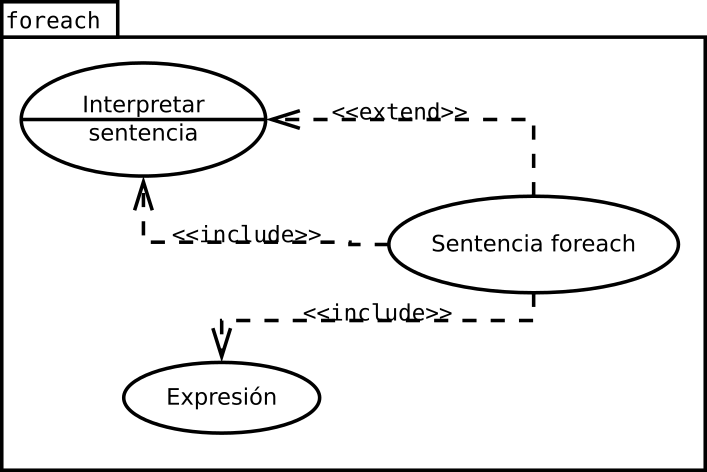
\includegraphics[scale=0.4]{foreach.png} \\
%~ \end{center}
%~ \begin{framed}
%~ \FloatBarrier
%~ \begin{description}
   %~ \item[Caso de Uso:]  Sentencia forearch.
   %~ \item [Tipo:] Sentencia.
   %~ \item[Nivel:]  Subfunción.
   %~ \item[Descripción:] 
   %~ Interpreta una sentencia foreach. Para ello valora la expresión de conjunto
   %~ y ejecuta el bloque de sentencias por cada uno de los elementos contenidos en el valor devuelto.
   %~ En cada iteración  el elemento será asignado a el identificador codificado en la sentencia foreach.
   %~ \item[Precondiciones:] 
   %~ La sentencia interpretada es una sentencia foreach.
   %~ \item[Postcondiciones:] 
   %~ La sentencia foreach queda interpretada.   
   %~ \item[Escenario principal:] \hfill
   %~ \begin{enumerate}
   %~ \item El sistema obtiene la expresión de conjunto.
   %~ \item Include (Expresión).
   %~ \item El sistema obtiene el primer elemento del valor de la expresión.
   %~ \item El sistema asigna el valor del elemento al identificador facilitado y obtiene el bloque de sentencias.
   %~ \item Include (Interprete) \\\\ \hfill
   %~ Se repite los pasos 3-4 por cada elemento en el valor de la expresión.
   %~ \end{enumerate}
   %~ \item[Flujo alternativo:] \hfill 
   %~ \begin{enumerate} \itemsep1pt \parskip0pt \parsep0pt
   %~ \setcounter{enumi}{2}
   %~ \renewcommand{\labelenumi}{}
   %~ \renewcommand{\labelenumiii}{\arabic{enumiii}.}
   %~ \renewcommand{\labelenumii}{\arabic{enumi}\alph{enumii}.}
      %~ \item 
      %~ \begin {enumerate}
         %~ \setcounter{enumii}{0}
         %~ \item La expresión resulta en un conjunto vacío.
         %~ \begin{enumerate}
         %~ \item El sistema no realiza ninguna acción.
         %~ \end{enumerate}
      %~ \end{enumerate}
   %~ \end{enumerate}
   %~ \begin{enumerate} \itemsep1pt \parskip0pt \parsep0pt
   %~ \setcounter{enumi}{2}
   %~ \renewcommand{\labelenumi}{}
   %~ \renewcommand{\labelenumiii}{\arabic{enumiii}.}
   %~ \renewcommand{\labelenumii}{\arabic{enumi}\alph{enumii}.}
      %~ \item 
      %~ \begin {enumerate}
         %~ \setcounter{enumii}{1}
         %~ \item La expresión es una cadena de caracteres.
         %~ \begin{enumerate}
         %~ \item Se toma como conjunto cada caracter en la cadena.
         %~ \end{enumerate}
      %~ \end{enumerate}
   %~ \end{enumerate}
   %~ \begin{enumerate} \itemsep1pt \parskip0pt \parsep0pt
   %~ \setcounter{enumi}{2}
   %~ \renewcommand{\labelenumi}{}
   %~ \renewcommand{\labelenumiii}{\arabic{enumiii}.}
   %~ \renewcommand{\labelenumii}{\arabic{enumi}\alph{enumii}.}
      %~ \item 
      %~ \begin {enumerate}
         %~ \setcounter{enumii}{2}
         %~ \item La expresión tiene un valor numérico.
         %~ \begin{enumerate}
         %~ \item Se toma como conjunto cada número entero desde 0 al valor entero
         %~ de la expresión.
         %~ \end{enumerate}
      %~ \end{enumerate}
   %~ \end{enumerate}
   %~ \begin{enumerate} \itemsep1pt \parskip0pt \parsep0pt
   %~ \setcounter{enumi}{2}
   %~ \renewcommand{\labelenumi}{}
   %~ \renewcommand{\labelenumiii}{\arabic{enumiii}.}
   %~ \renewcommand{\labelenumii}{\arabic{enumi}\alph{enumii}.}
      %~ \item 
      %~ \begin {enumerate}
         %~ \setcounter{enumii}{3}
         %~ \item La expresión tiene un valor lógico.
         %~ \begin{enumerate}
         %~ \item Si el valor es verdadero lo asigna al identificador y obtiene el bloque de sentencias
         %~ \item Include (Interpretar) \\ \\ \hfill
         %~ Repite el caso de uso.
         %~ \end{enumerate}
      %~ \end{enumerate}
   %~ \end{enumerate}
   %~ \begin{enumerate} \itemsep1pt \parskip0pt \parsep0pt
   %~ \setcounter{enumi}{2}
   %~ \renewcommand{\labelenumi}{}
   %~ \renewcommand{\labelenumiii}{\arabic{enumiii}.}
   %~ \renewcommand{\labelenumii}{\arabic{enumi}\alph{enumii}.}
      %~ \item 
      %~ \begin {enumerate}
         %~ \setcounter{enumii}{4}
         %~ \item La expresión tiene otro tipo de valor.
         %~ \begin{enumerate}
         %~ \item El sistema no realiza ninguna acción.
         %~ \end{enumerate}
      %~ \end{enumerate}
   %~ \end{enumerate}
%~ \end{description}
 %~ \FloatBarrier
%~ \end{framed}
%~ % ----------------------------------------------------------------------
%~ \subsubsection {Sentencia de iteración ágil}
%~ \begin{center}
%~ 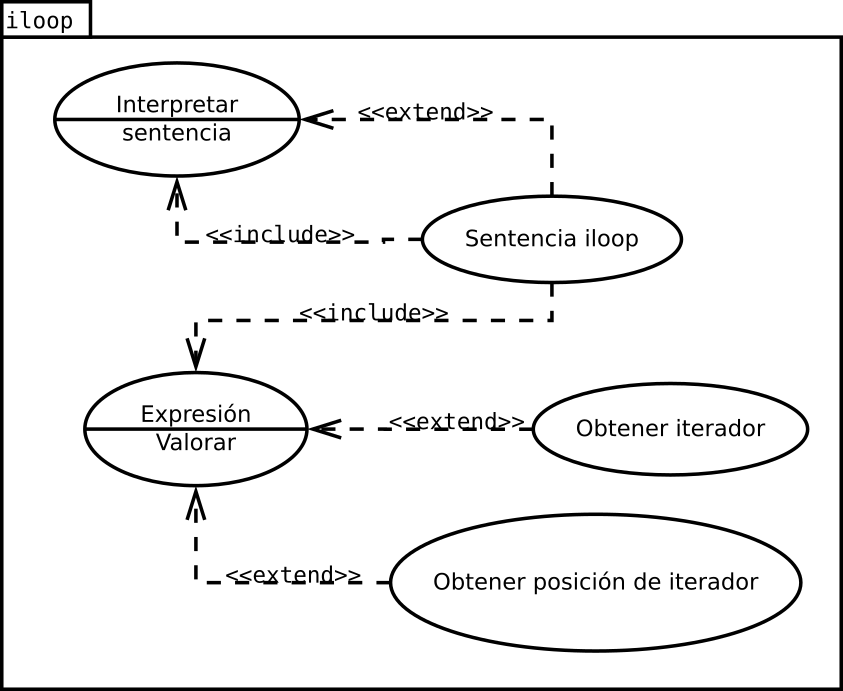
\includegraphics[scale=0.4]{iloop.png} \\
%~ \end{center}
%~ \begin{framed}
%~ \FloatBarrier
%~ \begin{description}
   %~ \item[Caso de Uso:]  Sentencia de iteración ágil.
   %~ \item [Tipo:] Sentencia.
   %~ \item[Nivel:]  Subfunción.
   %~ \item[Descripción:] 
   %~ Interpreta una sentencia de iteración ágil. Para ello valora la expresión de conjunto
   %~ y ejecuta el bloque de sentencias por cada uno de los elementos contenidos en el valor devuelto.
   %~ Cada elemento será asignado a una entidad denominada de iterador, también será asignada 
   %~ la posición del elemento en la secuencia a otra entidad denominada posición del iterador. 
   %~ \item[Precondiciones:] 
   %~ La sentencia interpretada es una sentencia de iteración ágil.
   %~ \item[Postcondiciones:] 
   %~ La sentencia de iteración ágil queda interpretada.   
   %~ \item[Escenario principal:] \hfill
   %~ \begin{enumerate}
   %~ \item El sistema obtiene la expresión de conjunto.
   %~ \item Include (Expresión).
   %~ \item El sistema obtiene el primer elemento del valor de la expresión.
   %~ \item El sistema asigna el valor del elemento al iterador y la posición del mismo a la posición del iterador, 
   %~ luego obtiene el bloque de sentencias para ser interpretadas.
   %~ \item Include (Interprete) \\\\ \hfill
   %~ Se repite los pasos 3-4 por cada elemento en el valor de la expresión.
   %~ \end{enumerate}
   %~ \item[Flujo alternativo:] \hfill 
   %~ \begin{enumerate} \itemsep1pt \parskip0pt \parsep0pt
   %~ \setcounter{enumi}{2}
   %~ \renewcommand{\labelenumi}{}
   %~ \renewcommand{\labelenumiii}{\arabic{enumiii}.}
   %~ \renewcommand{\labelenumii}{\arabic{enumi}\alph{enumii}.}
      %~ \item 
      %~ \begin {enumerate}
         %~ \setcounter{enumii}{0}
         %~ \item La expresión resulta en un conjunto vacío.
         %~ \begin{enumerate}
         %~ \item El sistema no realiza ninguna acción.
         %~ \end{enumerate}
      %~ \end{enumerate}
   %~ \end{enumerate}
   %~ \begin{enumerate} \itemsep1pt \parskip0pt \parsep0pt
   %~ \setcounter{enumi}{2}
   %~ \renewcommand{\labelenumi}{}
   %~ \renewcommand{\labelenumiii}{\arabic{enumiii}.}
   %~ \renewcommand{\labelenumii}{\arabic{enumi}\alph{enumii}.}
      %~ \item 
      %~ \begin {enumerate}
         %~ \setcounter{enumii}{1}
         %~ \item La expresión es una cadena de caracteres.
         %~ \begin{enumerate}
         %~ \item Se toma como conjunto cada carácter en la cadena.
         %~ \end{enumerate}
      %~ \end{enumerate}
   %~ \end{enumerate}
   %~ \begin{enumerate} \itemsep1pt \parskip0pt \parsep0pt
   %~ \setcounter{enumi}{2}
   %~ \renewcommand{\labelenumi}{}
   %~ \renewcommand{\labelenumiii}{\arabic{enumiii}.}
   %~ \renewcommand{\labelenumii}{\arabic{enumi}\alph{enumii}.}
      %~ \item 
      %~ \begin {enumerate}
         %~ \setcounter{enumii}{2}
         %~ \item La expresión tiene un valor numérico.
         %~ \begin{enumerate}
         %~ \item Se toma como conjunto cada número entero desde 0 al valor entero
         %~ de la expresión.
         %~ \end{enumerate}
      %~ \end{enumerate}
   %~ \end{enumerate}
   %~ \begin{enumerate} \itemsep1pt \parskip0pt \parsep0pt
   %~ \setcounter{enumi}{2}
   %~ \renewcommand{\labelenumi}{}
   %~ \renewcommand{\labelenumiii}{\arabic{enumiii}.}
   %~ \renewcommand{\labelenumii}{\arabic{enumi}\alph{enumii}.}
      %~ \item 
      %~ \begin {enumerate}
         %~ \setcounter{enumii}{3}
         %~ \item La expresión tiene un valor lógico.
         %~ \begin{enumerate}
         %~ \item Si el valor es verdadero lo asigna al iterador y se obtiene el bloque de sentencias
         %~ \item Include (Interpretar) \\ \\ \hfill
         %~ Repite el caso de uso.
         %~ \end{enumerate}
      %~ \end{enumerate}
   %~ \end{enumerate}
   %~ \begin{enumerate} \itemsep1pt \parskip0pt \parsep0pt
   %~ \setcounter{enumi}{2}
   %~ \renewcommand{\labelenumi}{}
   %~ \renewcommand{\labelenumiii}{\arabic{enumiii}.}
   %~ \renewcommand{\labelenumii}{\arabic{enumi}\alph{enumii}.}
      %~ \item 
      %~ \begin {enumerate}
         %~ \setcounter{enumii}{4}
         %~ \item La expresión tiene otro tipo de valor.
         %~ \begin{enumerate}
         %~ \item El sistema no realiza ninguna acción.
         %~ \end{enumerate}
      %~ \end{enumerate}
   %~ \end{enumerate}
%~ \end{description}
 %~ \FloatBarrier
%~ \end{framed}
%~ % ----
%~ \paragraph {Obtener iterador}
%~ \begin{framed}
%~ \FloatBarrier
%~ \begin{description}
   %~ \item[Caso de Uso:]  Obtener iterador.
   %~ \item [Tipo:] Expresión.
   %~ \item[Nivel:]  Subfunción.
   %~ \item[Descripción:] 
   %~ Accede al valor del iterador de una de las sentencias de iteración ágil que se pueden encontrar anidadas.  
   %~ La expresión puede codificar el índice de la sentencia de iteración ágil que se encuentra anidada y sobre la
   %~ cual se obtendrá el valor del iterador. El índice comienza en 0 y a partir de la última sentencia anidada.
   %~ \item[Precondiciones:] 
   %~ Se valora una expresión de acceso al iterador, además la expresión forma parte 
   %~ de una sentencia que se encuentra dentro del bloque de una sentencia de iteración ágil, o conjunto 
   %~ de estas anidas.
   %~ \item[Postcondiciones:] 
   %~ Se atribuye a la expresión el valor del iterador de la sentencia de iteración ágil 
   %~ indicada.   
   %~ \item[Escenario principal:] \hfill
   %~ \begin{enumerate}
   %~ \item El sistema obtiene y atribuye a la expresión el valor del iterador 
   %~ de la sentencia de iteración ágil indicada por el índice facilitado.
   %~ \end{enumerate}
   %~ \item[Flujo alternativo:] \hfill 
   %~ \begin{enumerate} \itemsep1pt \parskip0pt \parsep0pt
   %~ \setcounter{enumi}{0}
   %~ \renewcommand{\labelenumi}{}
   %~ \renewcommand{\labelenumiii}{\arabic{enumiii}.}
   %~ \renewcommand{\labelenumii}{\arabic{enumi}\alph{enumii}.}
      %~ \item 
      %~ \begin {enumerate}
         %~ \setcounter{enumii}{0}
         %~ \item No se ha facilitado un índice.
         %~ \begin{enumerate}
         %~ \item Se toma como índice el valor 0. 
         %~ \end{enumerate}
      %~ \end{enumerate}
   %~ \end{enumerate}
   %~ \begin{enumerate} \itemsep1pt \parskip0pt \parsep0pt
   %~ \setcounter{enumi}{0}
   %~ \renewcommand{\labelenumi}{}
   %~ \renewcommand{\labelenumiii}{\arabic{enumiii}.}
   %~ \renewcommand{\labelenumii}{\arabic{enumi}\alph{enumii}.}
      %~ \item 
      %~ \begin {enumerate}
         %~ \setcounter{enumii}{1}
         %~ \item No se encuentra una sentencia de iteración ágil en el índice dado.
         %~ \begin{enumerate}
         %~ \item El sistema informa del error y finaliza la interpretación del 
         %~ la sentencia.
         %~ \end{enumerate}
      %~ \end{enumerate}
   %~ \end{enumerate}
%~ \end{description}
 %~ \FloatBarrier
%~ \end{framed}
%~ % ----
%~ \paragraph {Obtener posición de iterador}
%~ \begin{framed}
%~ \FloatBarrier
%~ \begin{description}
   %~ \item[Caso de Uso:]  Obtener posición de iterador.
   %~ \item [Tipo:] Expresión.
   %~ \item[Nivel:]  Subfunción.
   %~ \item[Descripción:] 
   %~ Accede al valor de la posición del iterador de una de las sentencias de iteración ágil que se pueden encontrar anidadas.  
   %~ La expresión puede codificar el índice de la sentencia de iteración ágil que se encuentra anidada y sobre la
   %~ cual se obtendrá el valor de la posición del iterador. El índice comienza en 0 y a partir de la última sentencia anidada.
   %~ \item[Precondiciones:] 
   %~ Se valora una expresión de acceso a la posición del iterador, además la expresión forma parte 
   %~ de una sentencia que se encuentra dentro del bloque de una sentencia de iteración ágil, o conjunto 
   %~ de estas anidas.
   %~ \item[Postcondiciones:] 
   %~ Se atribuye a la expresión el valor de la posición del iterador de la sentencia de iteración ágil 
   %~ indicada.   
   %~ \item[Escenario principal:] \hfill
   %~ \begin{enumerate}
   %~ \item El sistema obtiene y atribuye a la expresión el valor de la posición del iterador 
   %~ de la sentencia de iteración ágil indicada por el índice facilitado.
   %~ \end{enumerate}
   %~ \item[Flujo alternativo:] \hfill 
   %~ \begin{enumerate} \itemsep1pt \parskip0pt \parsep0pt
   %~ \setcounter{enumi}{0}
   %~ \renewcommand{\labelenumi}{}
   %~ \renewcommand{\labelenumiii}{\arabic{enumiii}.}
   %~ \renewcommand{\labelenumii}{\arabic{enumi}\alph{enumii}.}
      %~ \item 
      %~ \begin {enumerate}
         %~ \setcounter{enumii}{0}
         %~ \item No se ha facilitado un índice.
         %~ \begin{enumerate}
         %~ \item Se toma como índice el valor 0. 
         %~ \end{enumerate}
      %~ \end{enumerate}
   %~ \end{enumerate}
   %~ \begin{enumerate} \itemsep1pt \parskip0pt \parsep0pt
   %~ \setcounter{enumi}{0}
   %~ \renewcommand{\labelenumi}{}
   %~ \renewcommand{\labelenumiii}{\arabic{enumiii}.}
   %~ \renewcommand{\labelenumii}{\arabic{enumi}\alph{enumii}.}
      %~ \item 
      %~ \begin {enumerate}
         %~ \setcounter{enumii}{1}
         %~ \item No se encuentra una sentencia de iteración ágil en el índice dado.
         %~ \begin{enumerate}
         %~ \item El sistema informa del error y finaliza la interpretación del 
         %~ la sentencia.
         %~ \end{enumerate}
      %~ \end{enumerate}
   %~ \end{enumerate}
%~ \end{description}
 %~ \FloatBarrier
%~ \end{framed}
%~ % ======================================================================
%~ \subsubsection {Sentencia break}
%~ \begin{center}
%~ 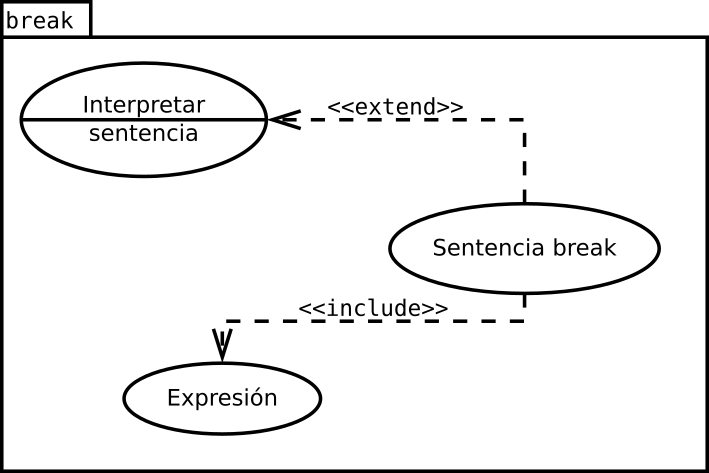
\includegraphics[scale=0.4]{break.png} \\
%~ \end{center}
%~ \begin{framed}
%~ \FloatBarrier
%~ \begin{description}
   %~ \item[Caso de Uso:]  Sentencia break.
   %~ \item [Tipo:] Sentencia.
   %~ \item[Nivel:]  Subfunción.
   %~ \item[Descripción:] 
   %~ Termina la interpretación de un bloque de sentencias o bloques de sentencias anidados. Adicionalmente
   %~ es posible indicar, codificado en forma de expresión, un índice que determina la posición del bloque de sentencias anidado cuya 
   %~ interpretación finalizará.
   %~ \item[Precondiciones:] 
   %~ La sentencia interpretada es una sentencia break y se encuentra dentro de un bloque de sentencias.
   %~ \item[Postcondiciones:] 
   %~ La sentencia break queda interpretada.
   %~ \item[Escenario principal:] \hfill
   %~ \begin{enumerate}
   %~ \item El sistema obtiene la expresión correspondiente al índice, que referencia el bloque que finalizará.
   %~ \item Include (Expresión).
   %~ \item El sistema finaliza la interpretación del bloque de sentencias indicado por el valor de la expresión. 
   %~ \item El sistema hace que la próxima sentencia que se interprete sea la siguiente al bloque.
   %~ \end{enumerate}
   %~ \item[Flujo alternativo:] \hfill 
   %~ \begin{enumerate} \itemsep1pt \parskip0pt \parsep0pt
   %~ \setcounter{enumi}{0}
   %~ \renewcommand{\labelenumi}{}
   %~ \renewcommand{\labelenumiii}{\arabic{enumiii}.}
   %~ \renewcommand{\labelenumii}{\arabic{enumi}\alph{enumii}.}
      %~ \item 
      %~ \begin {enumerate}
         %~ \setcounter{enumii}{0}
         %~ \item No se ha facilitado un índice.
         %~ \begin{enumerate}
         %~ \item Se toma como índice el valor 0. 
         %~ \end{enumerate}
      %~ \end{enumerate}
   %~ \end{enumerate}
   %~ \begin{enumerate} \itemsep1pt \parskip0pt \parsep0pt
   %~ \setcounter{enumi}{2}
   %~ \renewcommand{\labelenumi}{}
   %~ \renewcommand{\labelenumiii}{\arabic{enumiii}.}
   %~ \renewcommand{\labelenumii}{\arabic{enumi}\alph{enumii}.}
      %~ \item 
      %~ \begin {enumerate}
         %~ \setcounter{enumii}{0}
         %~ \item No se encuentra un bloque de sentencias en el índice dado.
         %~ \begin{enumerate}
         %~ \item El sistema informa del error y finaliza la interpretación del 
         %~ la sentencia.
         %~ \end{enumerate}
      %~ \end{enumerate}
   %~ \end{enumerate}
%~ \end{description}
 %~ \FloatBarrier
%~ \end{framed}
%~ % ======================================================================
%~ \subsubsection {Sentencia continue}
%~ \begin{center}
%~ 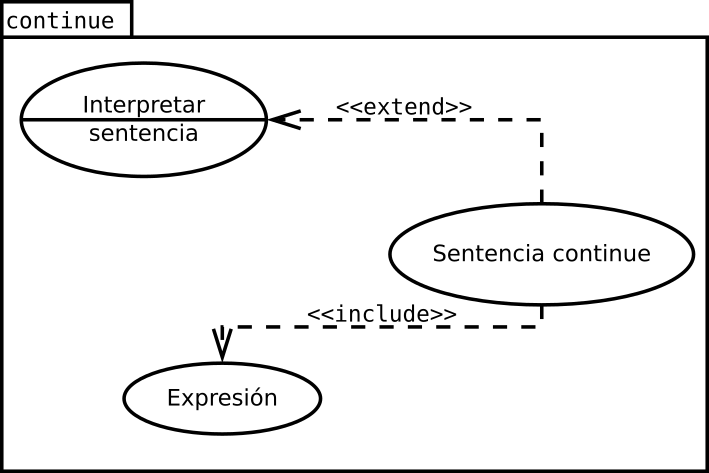
\includegraphics[scale=0.4]{continue.png} \\
%~ \end{center}
%~ \begin{framed}
%~ \FloatBarrier
%~ \begin{description}
   %~ \item[Caso de Uso:]  Sentencia continue.
   %~ \item [Tipo:] Sentencia.
   %~ \item[Nivel:]  Subfunción.
   %~ \item[Descripción:] 
   %~ Termina la iteración actual  de un bloque de sentencias iterativo o bloques de sentencias anidados. Adicionalmente
   %~ es posible indicar, codificado en forma de expresión, un índice que determina la posición del bloque de sentencias iterativa anidado cuya 
   %~ iteración actual finalizará.
   %~ \item[Precondiciones:] 
   %~ La sentencia interpretada es una sentencia continue y se encuentra dentro de un bloque de sentencias iterativo.
   %~ \item[Postcondiciones:] 
   %~ La sentencia continue queda interpretada.
   %~ \item[Escenario principal:] \hfill
   %~ \begin{enumerate}
   %~ \item El sistema obtiene la expresión correspondiente al índice, que referencia el bloque iterativo que finalizará.
   %~ \item Include (Expresión).
   %~ \item El sistema finaliza la iteración actual del bloque de sentencias indicado por el valor de la expresión. 
   %~ \item El sistema hace que la próxima sentencia sea la correspondiente al fin de iteración del bloque especificado.
   %~ \end{enumerate}
   %~ \item[Flujo alternativo:] \hfill 
   %~ \begin{enumerate} \itemsep1pt \parskip0pt \parsep0pt
   %~ \setcounter{enumi}{0}
   %~ \renewcommand{\labelenumi}{}
   %~ \renewcommand{\labelenumiii}{\arabic{enumiii}.}
   %~ \renewcommand{\labelenumii}{\arabic{enumi}\alph{enumii}.}
      %~ \item 
      %~ \begin {enumerate}
         %~ \setcounter{enumii}{0}
         %~ \item No se ha facilitado un índice.
         %~ \begin{enumerate}
         %~ \item Se toma como índice el valor 0. 
         %~ \end{enumerate}
      %~ \end{enumerate}
   %~ \end{enumerate}
   %~ \begin{enumerate} \itemsep1pt \parskip0pt \parsep0pt
   %~ \setcounter{enumi}{2}
   %~ \renewcommand{\labelenumi}{}
   %~ \renewcommand{\labelenumiii}{\arabic{enumiii}.}
   %~ \renewcommand{\labelenumii}{\arabic{enumi}\alph{enumii}.}
      %~ \item 
      %~ \begin {enumerate}
         %~ \setcounter{enumii}{0}
         %~ \item No se encuentra un bloque de sentencias iterativo en el índice dado.
         %~ \begin{enumerate}
         %~ \item El sistema informa del error y finaliza la interpretación del 
         %~ la sentencia.
         %~ \end{enumerate}
      %~ \end{enumerate}
   %~ \end{enumerate}
%~ \end{description}
 %~ \FloatBarrier
%~ \end{framed}
%~ % ----------------------------------------------------------------------
%~ \subsubsection {Sentencia try...catch [Aún por completar]}
%~ Aún por completar.
%~ \subsubsection {Sentencia throw [Aún por completar]}
%~ Aún por completar.
%~ \subsubsection {Sentencia with [Aún por completar]}
%~ Aún por completar.
%~ 
%~ \pagebreak
%~ 
%~ \subsection{Definiciones}
%~ \begin{center}
%~ 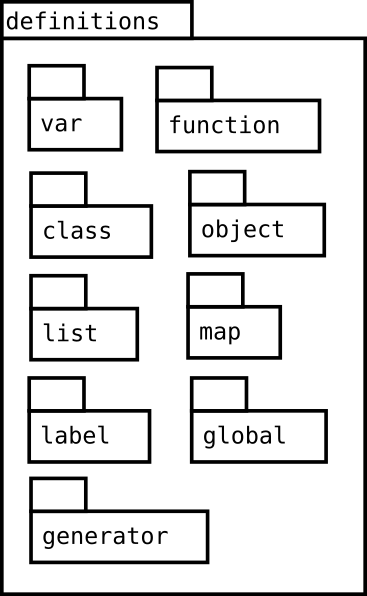
\includegraphics[scale=0.4]{definitions.png} \\
%~ \end{center}
%~ \subsubsection {Variable}
%~ \begin{center}
%~ 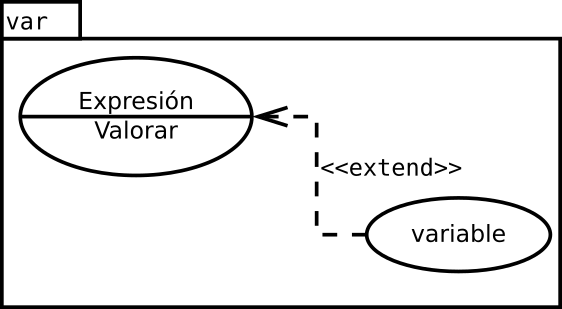
\includegraphics[scale=0.4]{id.png} \\
%~ \end{center}
%~ \begin{framed}
%~ \FloatBarrier
%~ \begin{description}
   %~ \item[Caso de Uso:]  Variable.
   %~ \item [Tipo:] Expresiones.
   %~ \item[Nivel:]  Subfunción.
   %~ \item[Descripción:] 
   %~ El sistema valora la expresión accediendo al valor guardado en la variable que se corresponde con el identificador 
   %~ codificado.
   %~ \item[Precondiciones:] 
   %~ El sistema se encuentra valorando una expresión.
   %~ \item[Postcondiciones:] 
   %~ A la expresión se le atribuye el valor asociado con el identificador. 
   %~ \item[Escenario principal:] \hfill
   %~ \begin{enumerate}
   %~ \item El sistema obtiene el valor asociado al identificador codificado y se lo atribuye 
   %~ a la expresión.
   %~ \end{enumerate}
   %~ \item[Flujo alternativo:] \hfill 
   %~ \begin{enumerate} \itemsep1pt \parskip0pt \parsep0pt
   %~ \setcounter{enumi}{0}
   %~ \renewcommand{\labelenumi}{}
   %~ \renewcommand{\labelenumiii}{\arabic{enumiii}.}
   %~ \renewcommand{\labelenumii}{\arabic{enumi}\alph{enumii}.}
      %~ \item 
      %~ \begin {enumerate}
         %~ \setcounter{enumii}{0}
         %~ \item El identificador no tiene valor asociado.
         %~ \begin{enumerate}
         %~ \item Se toma valor nulo. 
         %~ \end{enumerate}
      %~ \end{enumerate}
   %~ \end{enumerate}
%~ \end{description}
 %~ \FloatBarrier
%~ \end{framed}


\subsubsection{Iniciar interpretación red} 

\begin{description}
   \item[Caso de Uso:]  Iniciar interpretación red 
   \item [Tipo:] Red
   \item[Descripción:] 
   Un sistema externo inicia una interpretación por red, estableciendo el contenido fuente que será interpretado.
   El sistema procesa la petición y abre un nuevo proceso de interpretación por pasos.
   \item[Precondiciones:] 
   No tiene. 
   \item[Postcondiciones:] 
   Se establece el código fuente a interpretar y se inicia una interpretación por pasos.
   \item[Escenario principal:] \hfill
   \begin{enumerate}
   \item El sistema espera una petición de interpretación por red.
   \item El sistema externo inicia la comunicación y facilita el código fuente.
   \item El sistema establece el código fuente y abre un nuevo proceso de interpretación por pasos. 
   \end{enumerate}
   \item[Flujo alternativo:] \hfill 
   %~ \begin{enumerate} \itemsep1pt \parskip0pt \parsep0pt
   %~ \setcounter{enumi}{3}
   %~ \renewcommand{\labelenumi}{}
   %~ \renewcommand{\labelenumiii}{\arabic{enumiii}.}
   %~ \renewcommand{\labelenumii}{\arabic{enumi}\alph{enumii}.}
      %~ \item 
      %~ \begin {enumerate}
         %~ \setcounter{enumii}{0}
         %~ \item El código fuente no presenta una sintaxis OMI correcta.
         %~ \begin{enumerate}
         %~ \item Se devuelve un estado de error.
         %~ \end{enumerate}
      %~ \end{enumerate}
   %~ \end{enumerate}
   \begin{enumerate} \itemsep1pt \parskip0pt \parsep0pt
   \setcounter{enumi}{0}
   \renewcommand{\labelenumi}{}
   \renewcommand{\labelenumiii}{\arabic{enumiii}.}
   \renewcommand{\labelenumii}{\arabic{enumi}\alph{enumii}.}
      \item 
      \begin {enumerate}
         \setcounter{enumii}{0}
         \item El servicio no se encuentra disponible.
         \begin{enumerate}
         \item Se devuelve un estado de error.
         \end{enumerate}
      \end{enumerate}
   \end{enumerate}
\end{description}


\subsubsection{Obtener pasos interpretación red} 

\begin{description}
   \item[Caso de Uso:]  Obtener pasos interpretación red 
   \item [Tipo:] Red
   \item[Descripción:] 
   Un sistema externo obtiene un nuevo estado dentro de los pasos en el proceso de
   interpretación del código fuente establecido.
   \item[Precondiciones:] 
   Se ha establecido código fuente para una interpretación por pasos.
   \item[Postcondiciones:] 
   Se lleva a cabo un nuevo paso dentro del proceso de interpretación. Obteniéndose el 
   siguiente estado.
   \item[Escenario principal:] \hfill
   \begin{enumerate}
   \item El sistema espera la petición de un nuevo paso en una iterpretación por red.
   \item El sistema externo realiza la petición de un nuevo paso.
   \item Incluir (Interpretar).
   \item El sistema devuelve una estructura de datos que representa 
   el estado actual del proceso de interpretación.
   \end{enumerate}
   \item[Flujo alternativo:] \hfill 
   %~ \begin{enumerate} \itemsep1pt \parskip0pt \parsep0pt
   %~ \setcounter{enumi}{3}
   %~ \renewcommand{\labelenumi}{}
   %~ \renewcommand{\labelenumiii}{\arabic{enumiii}.}
   %~ \renewcommand{\labelenumii}{\arabic{enumi}\alph{enumii}.}
      %~ \item 
      %~ \begin {enumerate}
         %~ \setcounter{enumii}{0}
         %~ \item El código fuente no presenta una sintaxis OMI correcta.
         %~ \begin{enumerate}
         %~ \item Se devuelve un estado de error.
         %~ \end{enumerate}
      %~ \end{enumerate}
   %~ \end{enumerate}
   \begin{enumerate} \itemsep1pt \parskip0pt \parsep0pt
   \setcounter{enumi}{0}
   \renewcommand{\labelenumi}{}
   \renewcommand{\labelenumiii}{\arabic{enumiii}.}
   \renewcommand{\labelenumii}{\arabic{enumi}\alph{enumii}.}
      \item 
      \begin {enumerate}
         \setcounter{enumii}{0}
         \item El servicio no se encuentra disponible.
         \begin{enumerate}
         \item Se devuelve un estado de error.
         \end{enumerate}
      \end{enumerate}
   \end{enumerate}
   \begin{enumerate} \itemsep1pt \parskip0pt \parsep0pt
   \setcounter{enumi}{2}
   \renewcommand{\labelenumi}{}
   \renewcommand{\labelenumiii}{\arabic{enumiii}.}
   \renewcommand{\labelenumii}{\arabic{enumi}\alph{enumii}.}
      \item 
      \begin {enumerate}
         \setcounter{enumii}{0}
         \item El código fuente presenta errores sintáctico o léxicos.
         \begin{enumerate}
         \item Se devuelve un estado de error. 
         \end{enumerate}
      \end{enumerate}
   \end{enumerate}
\end{description}



% ----------------------------------------------------------------------
\subsection {runTree}
\begin{center}
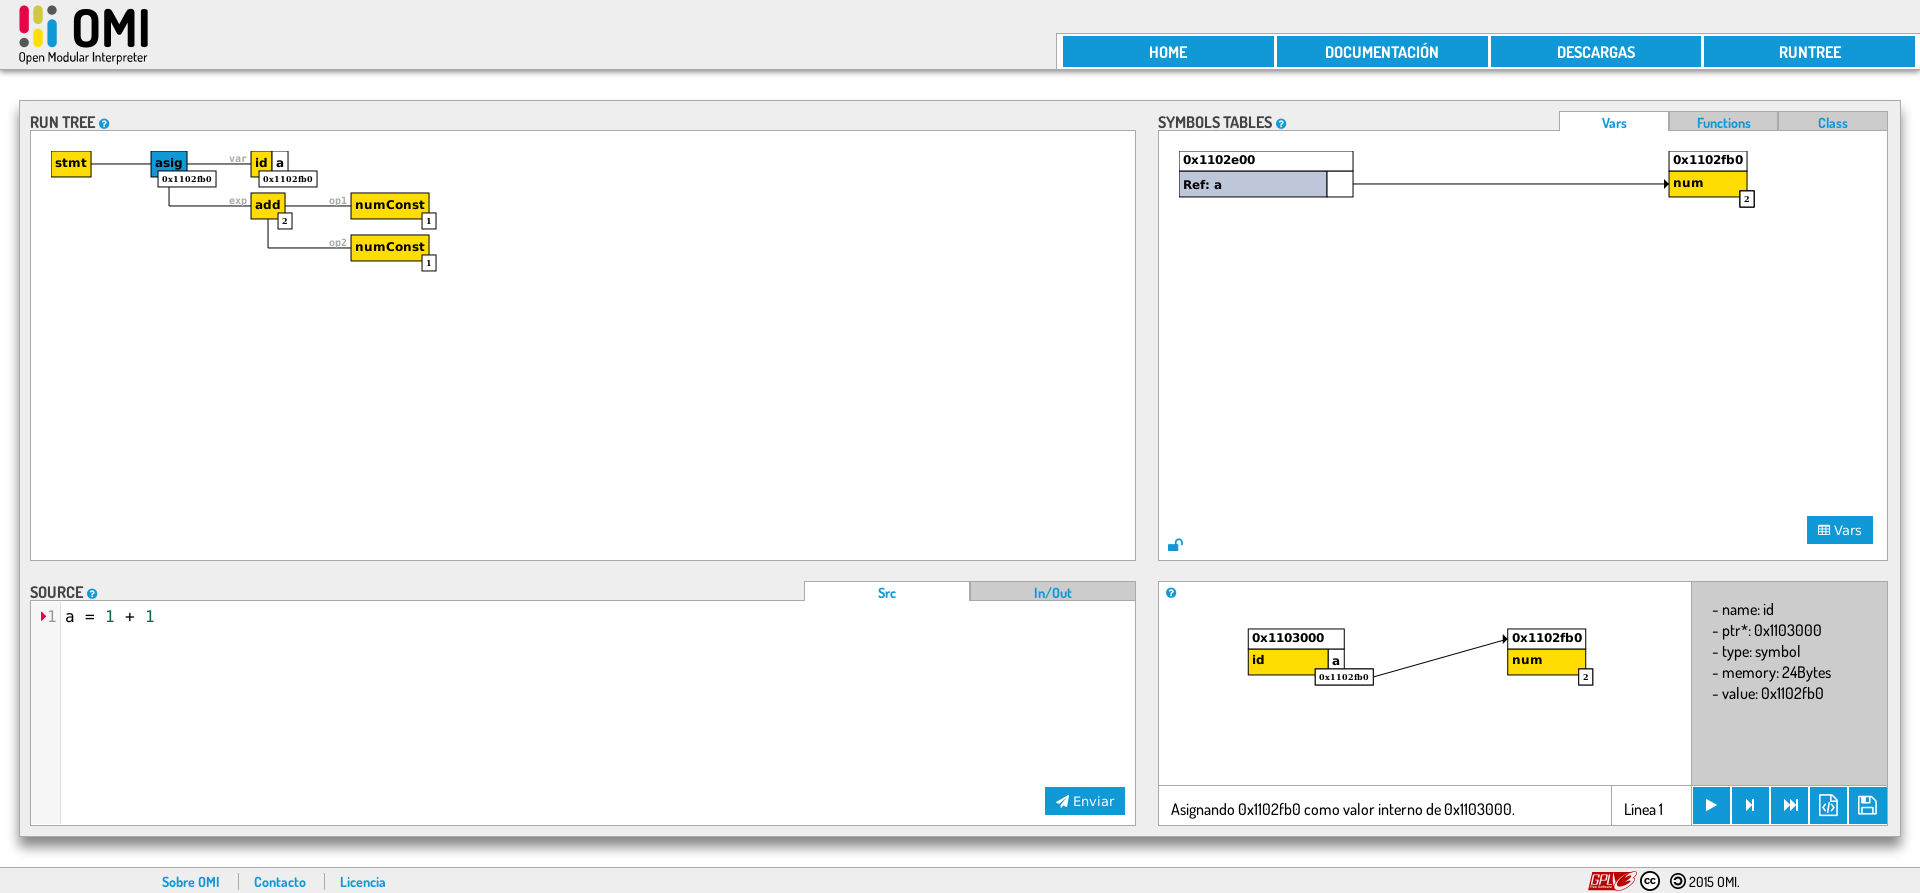
\includegraphics[scale=0.5]{runtree.png} \\
\end{center}
\subsubsection{Enviar código fuente} 

\begin{description}
   \item[Caso de Uso:]  Enviar código fuente 
   \item [Tipo:] runTree
   \item[Descripción:] 
   El usuario envía  texto correspondiente a código fuente para su interpretación y análisis. 
   El sistema cliente envía el código al servidor que lo establecerá como fuente a interpretar y enviará
   datos relativos al proceso.
   El cliente imprime el árbol sintáctico y espera acciones del usuario.
   \item[Precondiciones:] 
   No tiene.
   \item[Postcondiciones:] 
   Se ha establecido el código fuente para el análisis del proceso de interpretación y se ha imprimido el árbol sintáctico. 
   \item[Escenario principal:] \hfill
   \begin{enumerate}
   \item El sistema solicita  código fuente escrito en OMI.
   \item El usuario introduce código fuente escrito en el lenguaje OMI.
   \item El sistema cliente runtree envía el código fuente al servidor para su interpretación.
   \item El sistema servidor devuelve una representación de los datos que describen el árbol sintáctico relativo al código fuente enviado.
   \item El sistema cliente imprime el árbol sintáctico. 
   \end{enumerate}
   \item[Flujo alternativo:] \hfill 
   \begin{enumerate} \itemsep1pt \parskip0pt \parsep0pt
   \setcounter{enumi}{3}
   \renewcommand{\labelenumi}{}
   \renewcommand{\labelenumiii}{\arabic{enumiii}.}
   \renewcommand{\labelenumii}{\arabic{enumi}\alph{enumii}.}
      \item 
      \begin {enumerate}
         \setcounter{enumii}{0}
         \item El código fuente no presenta una sintaxis OMI correcta.
         \begin{enumerate}
         \item Se devuelve un estado de error.
         \end{enumerate}
      \end{enumerate}
   \end{enumerate}
   \begin{enumerate} \itemsep1pt \parskip0pt \parsep0pt
   \setcounter{enumi}{3}
   \renewcommand{\labelenumi}{}
   \renewcommand{\labelenumiii}{\arabic{enumiii}.}
   \renewcommand{\labelenumii}{\arabic{enumi}\alph{enumii}.}
      \item 
      \begin {enumerate}
         \setcounter{enumii}{1}
         \item El servicio no se encuentra disponible.
         \begin{enumerate}
         \item Se devuelve un estado de error.
         \end{enumerate}
      \end{enumerate}
   \end{enumerate}
\end{description}


\subsubsection{Siguiente paso} 

\begin{description}
   \item[Caso de Uso:] Siguiente paso
   \item [Tipo:] runTree
   \item[Descripción:] 
   El usuario usuario solicita un nuevo paso en el proceso de interpretación. 
   El sistema cliente obtiene el nuevo paso del servidor y lo representa en pantalla.
   \item[Precondiciones:] \hfill 
   \begin{itemize}
   \item Existe un código fuente establecido para estudio. 
   \item El estado actual del proceso no es final.
   \item La ejecución automática se encuentra desactivada. 
   \end{itemize}
   \item[Postcondiciones:] 
   Se representa en nuevo paso. 
   \item[Escenario principal:] \hfill
   \begin{enumerate}
   \item El usuario solicita un nuevo paso en el proceso de interpretación
   \item El sistema cliente solicita la resolución de un nuevo paso y representa
   el nuevo estado en pantalla. 
   \end{enumerate}
   \item[Flujo alternativo:] \hfill 
   \begin{enumerate} \itemsep1pt \parskip0pt \parsep0pt
   \setcounter{enumi}{1}
   \renewcommand{\labelenumi}{}
   \renewcommand{\labelenumiii}{\arabic{enumiii}.}
   \renewcommand{\labelenumii}{\arabic{enumi}\alph{enumii}.}
      \item 
      \begin {enumerate}
         \setcounter{enumii}{0}
         \item El servicio no se encuentra disponible.
         \begin{enumerate}
         \item Se devuelve un estado de error.
         \end{enumerate}
      \end{enumerate}
   \end{enumerate}
\end{description}


\subsubsection{Siguiente sentencia} 

\begin{description}
   \item[Caso de Uso:] Siguiente sentencia
   \item [Tipo:] runTree
   \item[Descripción:] 
   El usuario solicita la resolución de la siguiente sentencia. 
   El sistema cliente obtiene el estado correspondiente a la interpretación de la siguiente sentencia 
   dentro del proceso de interpretación y lo representa en pantalla.
  \item[Precondiciones:] \hfill 
   \begin{itemize}
   \item Existe un código fuente establecido para estudio. 
   \item El estado actual del proceso no es final.
   \item La ejecución automática se encuentra desactivada. 
   \end{itemize}
   \item[Postcondiciones:] 
   Se representa en nuevo estado correspondiente a la interpretación de una sentencia completa. 
   \item[Escenario principal:] \hfill
   \begin{enumerate}
   \item El usuario solicita la resolución de una nueva senterncia en el proceso de interpretación.
   \item El sistema cliente solicita la resolución de la sentencia completa y representa
   el nuevo estado en pantalla. 
   \end{enumerate}
   \item[Flujo alternativo:] \hfill 
   \begin{enumerate} \itemsep1pt \parskip0pt \parsep0pt
   \setcounter{enumi}{1}
   \renewcommand{\labelenumi}{}
   \renewcommand{\labelenumiii}{\arabic{enumiii}.}
   \renewcommand{\labelenumii}{\arabic{enumi}\alph{enumii}.}
      \item 
      \begin {enumerate}
         \setcounter{enumii}{0}
         \item El servicio no se encuentra disponible.
         \begin{enumerate}
         \item Se devuelve un estado de error.
         \end{enumerate}
      \end{enumerate}
   \end{enumerate}
\end{description}


\subsubsection{Activar ejecución automática} 

\begin{description}
   \item[Caso de Uso:] Activar ejecución automática
   \item [Tipo:] runTree
   \item[Descripción:] 
   El usuario solicita la ejecución automática. 
   El sistema cliente obtiene y representa cada paso dentro del proceso 
   de interpretación hasta obtenerse un estado final.
   \item[Precondiciones:] \hfill 
   \begin{itemize}
   \item Existe un código fuente establecido para estudio. 
   \item El estado actual del proceso no es final.
   \item La ejecución automática se encuentra desactivada. 
   \end{itemize}
   \item[Postcondiciones:] 
   Se obtiene un estado final.
   \item[Escenario principal:] \hfill
   \begin{enumerate}
   \item El usuario activa la ejecución automática.
   \item El sistema obtiene y representa cada paso en el proceso de interpretación hasta que se 
   obtiene un estado final.
   \end{enumerate}
   \item[Flujo alternativo:] \hfill 
   \begin{enumerate} \itemsep1pt \parskip0pt \parsep0pt
   \setcounter{enumi}{1}
   \renewcommand{\labelenumi}{}
   \renewcommand{\labelenumiii}{\arabic{enumiii}.}
   \renewcommand{\labelenumii}{\arabic{enumi}\alph{enumii}.}
      \item 
      \begin {enumerate}
         \setcounter{enumii}{0}
         \item El servicio no se encuentra disponible.
         \begin{enumerate}
         \item Se devuelve un estado de error.
         \end{enumerate}
      \end{enumerate}
   \end{enumerate}
\end{description}


\subsubsection{Desactivar ejecución automática} 

\begin{description}
   \item[Caso de Uso:] Desactivar ejecución automática
   \item [Tipo:] runTree
   \item[Descripción:] 
   El usuario solicita la detención de la ejecución automática. 
   El sistema cliente detiene la ejecución automática y representa el estado actual.
   \item[Precondiciones:] \hfill 
   \begin{itemize}
   \item Existe un código fuente establecido para estudio. 
   \item El estado actual del proceso no es final.
   \item La ejecución automática se encuentra activada.
   \end{itemize}
   \item[Postcondiciones:] 
   Se obtiene el estado actual del proceso.
   \item[Escenario principal:] \hfill
   \begin{enumerate}
   \item El usuario desactiva la ejecución automática.
   \item El sistema cliente para la ejecución automática y representa el estado actual 
   \end{enumerate}
\end{description}


\subsubsection{Limpiar salida} 

\begin{description}
   \item[Caso de Uso:] Limpiar salida
   \item [Tipo:] runTree
   \item[Descripción:] 
   El usuario solicita la limpieza de los datos de salida. 
   El sistema cliente elimina la información disponible en la consola de salida.
   \item[Precondiciones:]
   No tiene.
   \item[Postcondiciones:] 
   La consola de salida queda vacía.
   \item[Escenario principal:] \hfill
   \begin{enumerate}
   \item El usuario solicita la limpieza de la salida.
   \item El sistema cliente limpia la información disponible en la consola de salida.  
   \end{enumerate}
\end{description}


\subsubsection{Ver información de nodo} 

\begin{description}
   \item[Caso de Uso:] Ver información de nodo.
   \item [Tipo:] runTree
   \item[Descripción:] 
   El usuario marca un nodo para ver su información.  
   El sistema cliente muestra la información relativa al nodo.
   \item[Precondiciones:]
   Existe un código fuente establecido para estudio. 
   \item[Postcondiciones:] 
   Se muestra información relativa al nodo.
   \item[Escenario principal:] \hfill
   \begin{enumerate}
   \item El usuario marca un nodo para ver su información.
   \item El sistema muestra información relativa al nodo tal como su 
   posición de memoria interna, su tamaño, su tipo y su nombre.  
   \end{enumerate}
\end{description}


\subsubsection{Ver contenido de la tabla de símbolos} 

\begin{description}
   \item[Caso de Uso:] Ver contenido de la tabla de símbolos.
   \item [Tipo:] runTree
   \item[Descripción:] 
   El usuario marca una tabla de símbolos para ver su contenido.  
   El sistema cliente muestra la información relativa a la tabla de símbolos.
   \item[Precondiciones:]
   Existe un código fuente establecido para estudio. 
   \item[Postcondiciones:] 
   Se muestra información relativa a la tabla de símbolos.
   \item[Escenario principal:] \hfill
   \begin{enumerate}
   \item El usuario indica una tabla de símbolos para ver su contenido.
   \item El sistema cliente muestra los nodos referenciados desde la tabla de
   símbolos dada.
   \end{enumerate}
\end{description}


\subsubsection{Guardar código fuente} 

\begin{description}
   \item[Caso de Uso:] Guardar código fuente.
   \item [Tipo:] runTree
   \item[Descripción:] 
   El usuario solicita guardar el codigo fuente escrito en un fichero local y el cliente
   abre el cuadro de diálogo correspondiente.
   \item[Precondiciones:]
   Existe un código escrito en el cliente 
   \item[Postcondiciones:] 
   Se guarda el código fuente en un fichero local.
   \item[Escenario principal:] \hfill
   \begin{enumerate}
   \item El usuario solicita guardar el código fuente en un fichero local.
   \item El sistema abre el cuadro de diálogo correspondiente.
   \end{enumerate}
\end{description}


\subsubsection{Abrir código fuente} 

\begin{description}
   \item[Caso de Uso:] Abrir código fuente.
   \item [Tipo:] runTree
   \item[Descripción:] 
   El usuario solicita cargar código fuente desde un fichero local.
   \item[Precondiciones:]
   No tiene.
   \item[Postcondiciones:] 
   Se carga el código fuente contenido en el fichero.
   \item[Escenario principal:] \hfill
   \begin{enumerate}
   \item El usuario solicita abrir un fichero de código fuente.
   \item El sistema abre el cuadro de diálogo correspondiente.
   \item El sistama carga el contenido del código fuente.
   \end{enumerate}
    \item[Flujo alternativo:] \hfill 
   \begin{enumerate} \itemsep1pt \parskip0pt \parsep0pt
   \setcounter{enumi}{1}
   \renewcommand{\labelenumi}{}
   \renewcommand{\labelenumiii}{\arabic{enumiii}.}
   \renewcommand{\labelenumii}{\arabic{enumi}\alph{enumii}.}
      \item 
      \begin {enumerate}
         \setcounter{enumii}{2}
         \item El fichero no contiene código en texto plano.
         \begin{enumerate}
         \item Se devuelve un estado de error.
         \end{enumerate}
      \end{enumerate}
   \end{enumerate}
\end{description}



\end{document}
%%%%%%%%%%%%%%%%%%%%%%%%%%%%%%%%%%%%%%%%%%%%%%%%%%%%%%%%%%%%%%%%%%%%%%%%
%Fco. Javier Bohórquez Ogalla
